\chapter{Language Statistics}\label{sec:lang_stat}
\epigraph{In trying to give an account of the statistical properties of language,
one is faced with the problem of having to find the common thread which would
show the many and multifarious forms of language statistics - embodied in scattered
papers written by linguists, philosophers, mathematicians, engineers, each using his 
own professional idiom - as belonging to one great whole: quantitative linguistics.}{Gustav Herdan (1966)}

% total from short-gutenber database
% n. types: 164,444
% n. tokens : 14,285,332
% 
% 
% found in CMU
% n. types : 46,094
% n. tokens: 13,481,254
%
% merriam-webster has more than 470,000 
% wikitionary 2,030,838 entries
If we agree to see language as a purpose driven stochastic event, 
it is important to view its statistics and observe how it is structured. 
We might stipulate that language is a usage driven process, 
the way it is used is shaped by its structures,
%the very fact of its usage is modeled according to way it is structured, 
and the way it is structured is dictated by its usage. 
We see language then as a dynamic process in a constant feedback loop.

To understand the statistical properties and build models of languages is a central task in understanding
how language works and create natural language processing systems. Traditionally, language has
been studied and modeled manually, describing each observation and building a language grammar from them.
With the recent availability of a massive amount of data, statistically trained models are an attractive
alternative. Probabilistic models of language are also fundamental in speech recognition systems to
resolve ambiguity situations, and might also be used in optical character recognition, handwriting recognition,
spelling correction, part-of-speech tagging, and machine translation.


``One striking clue to the importance of probabilities in language comes
from the wealth of frequency effects that pervade language representation, processing, and language change.
(...) Frequent words are recognized faster than infrequent words, and there is a bias toward interpreting 
ambiguous words in terms of their more frequent meanings. Frequent words lead leniting changes and 
are more prone to reduction in speech. Frequent combinations of phonemes and structures are perceived as
more grammatical, or well formed, than infrequent combinations. 
The relative frequency of derived words and their bases affects the morphological decomposability of complex words'' 
\citep{bod2003}.

It is important to understand how frequency affects language processes and how the various
aspects of the cognition processes are driven and self-organized by usage.  
Humans seem to track, record and exploit the occurrences of various kinds of events.
This might make it fundamental to understand the statistical properties of language
to better understand how a language works.
\cite{pierrehumbert2003} proposes that linguistics constraints are a result of statistical robust generalizations
that might be effectively learned, transmitted and exploited.
The symbolic concept of a phoneme is a probabilistic distribution over a continuous phonetic space.
The process of learning, recognition and classification of phonetic exemplars is a task
of adjusting the phonemic membership functions. Under this point o view, language is a probabilistic process.
Knowlegde of phonotatics involves knowledge of co-occurence probabilities of phonemes, and the well-formedness
of a string of phonemes is just a combined product of the contributions of its subparts.
``Such phonotactic probabilities are exploited in speech perception for segmentation,
and they affect well-formedness judgments, influence pronunciation, and
affect behavior in linguistic tasks such as creating blends'' \citep{bod2003}.

The effect and influence of probabilities on Language is present at different levels.
\cite{baayen2003} presented the influence of the frequency of occurrence at the morpheme level,
showing that the individual's choice among concurring affixes is strongly biased by the frequency
of occurrence of these affixes. At the word level, the processing and representation of words
is strongly influenced by lexical frequency and this behavior is independent of morphological
composition of words. This frequency effect is manifested in ambiguity resolution,
phoneme reduction, language change and speed of access \citep{bod2003}.
Individuals also track the co-occurrence of words, what influences speech comprehension 
and production. \cite{jurafsky2003} argues that more frequent word pairs have a shorter processing time and
may also suffer a phonetic reduction. Low-probability words (regarding the surroundings)
are more likely to receive a pitch accent. \cite{jurafsky2003} provide evidence that 
``people track the probabilities of syntactic structures'', what influences the processing time
of sentences and structures, and it is also involved in disambiguation.

``Language displays all the hallmarks of a probabilistic system. Categories
and well-formedness are gradient, and frequency effects are everywhere.
We believe all evidence points to a probabilistic language faculty.
Knowledge of language should be understood not as a minimal set of
categorical rules or constraints, but as a (possibly redundant) set of gradient 
rules, which may be characterized by a statistical distribution'' \citep{bod2003}.

As remarked by \cite{sedelow1966}, ``the study of patterns formed in the process of the
linguistic encoding of information, is of importance to any major research focusing upon
or dependent upon the production or analysis of language''. An increased interest on
the statistical and numerical counts of linguistics objects is perceived on Languages research,
where the \textit{quantitative} aspects have gained an important status. The use of 
computational resource and the availability of digital information has made the quantitative analysis 
task possible, what was hitherto unfeasible.

The quantitative analysis is also the basis of \textit{stylometrics} (quantitative stylistics)
which deals with the analysis from the standpoint of individual or functional style.
Style is regarded as a probabilistic concept by which selection
(choice), conscious or unconscious, is responsible for creating a style,
an emergent feature during the choice process in a universe of multiple
alternatives for expressing an idea \citep{tuldava2004}.
The analysis of emergent patterns in communication and the influence on the linguistic style 
used is analyzed by \cite{hancock2004} to investigate the truthful and deceptive
dyadic communication. The studies show that ``senders used more words overall,
increased references to others, and used more sense-based descriptions (e.g., seeing, touching) when lying as compared
to telling the truth. Receivers naïve to the deception manipulation produced more words and sense terms, and
asked more questions with shorter sentences when they were being lied to than when they were being told the truth''
\citep{hancock2004}.



The first remarkable study in the statistics of languages was done by George Kingsley Zipf, 
linguistic professor of Harvard, during the 1920s and 1930s. Zipf and his students performed many 
word count experiments and determined that there is a relationship between the word's frequency of 
appearance in texts and its rank, the product of them is roughly a constant. 
%That means, the most frequent word occurs twice as often as the second most frequent word; which occurs twice as often as the fourth most frequent word, and so forth. 
That means, the distribution follows a power law: $f(k;s,N) = C k^{-s}$, where $f$ stands for frequency, 
$C$ is a constant, $k$ is the word rank, $s$ the slope, the exponent characterizing the distribution, 
and $N$ is the number of elements in the set. Zipf's law is not, in fact, a law in the rigorous
sense, but an empirical observation that has an apparent robustness.

%As the number of occurrences cannot be a fractional number, we ought to find the constant $C$. 
The constant $C$ is a normalizing constant that might be found by calculating 
%Let's consider then 
the total number occurrences of all elements:
\begin{equation}
\sum_{k=1}^{N} f(k;s,N) = \sum_{n=1}^{N} C n^{-s} \textmd{ .}
\end{equation}
Normalizing the occurrences of each element ranked $k$ by the total of occurrences, leads us to
\begin{equation}
\label{eq:zipflaw}
f(k;s,N) = \frac{k^{-s}}{\sum_{n=1}^{N} n^{-s}} \textmd{ ,}
\end{equation}
that means, the constant $C$ is given by
\begin{equation}
C = \frac{1}{\sum_{n=1}^{N} n^{-s}} \textmd{ .}
\end{equation}

\begin{figure}[h!]
\centering
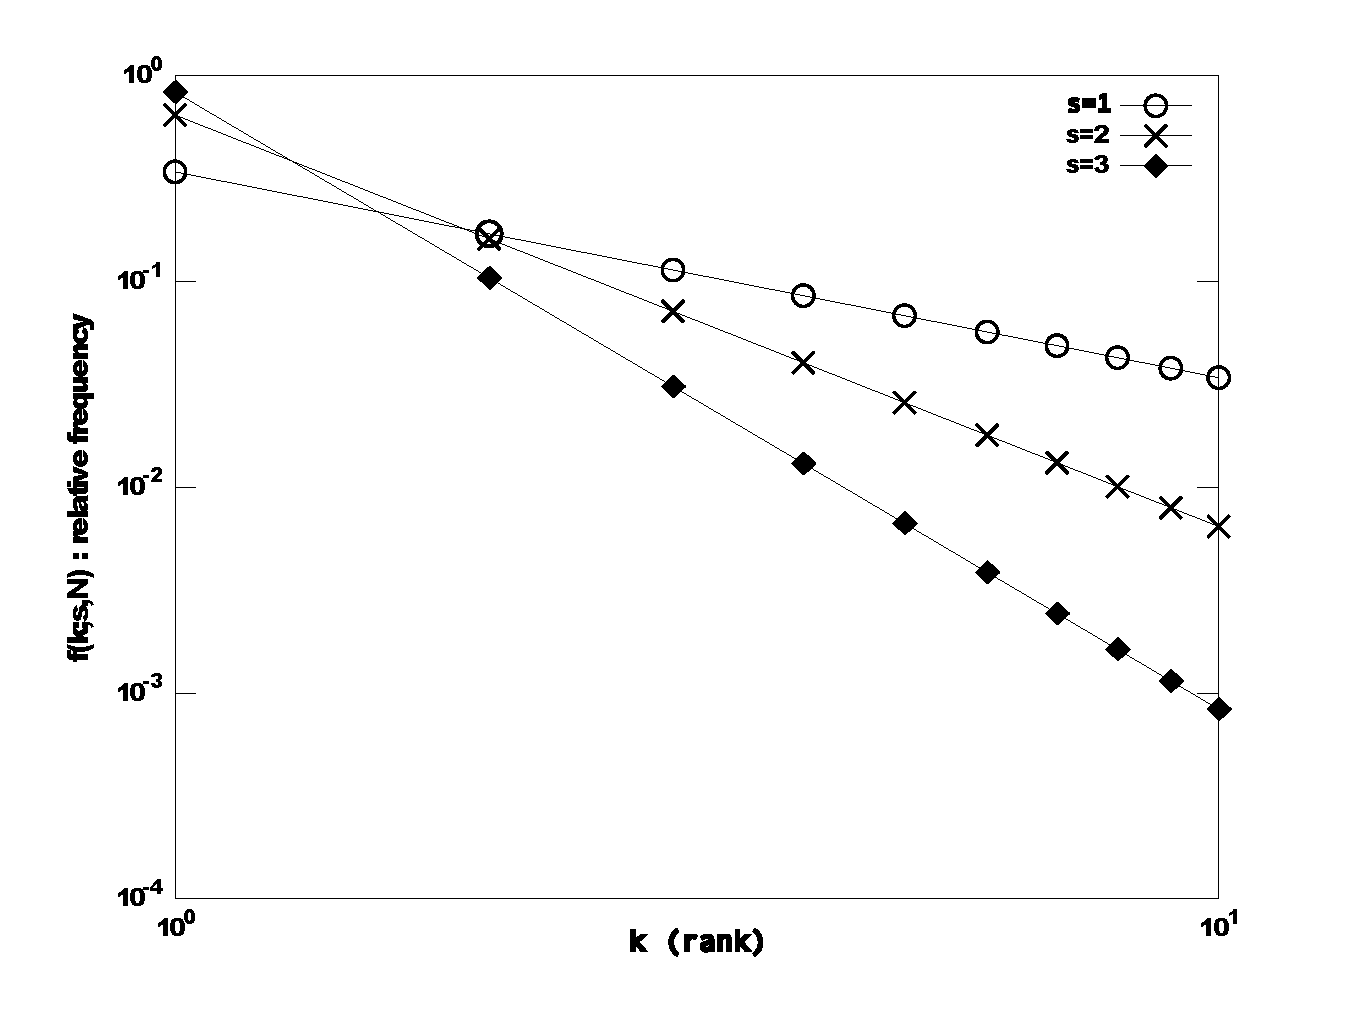
\includegraphics[width=0.75\textwidth]{images/zipf_pmf.pdf}
\caption{Zipf probability mass function for $N=10$ on a log-log scale for different values of $s$.}
\label{fig:zipf_pmf}
\end{figure} 

Zipf developed the idea of using an intrinsic linguistic or psychological reason to explain this phenomenon observed in the world of words. He named his theory the `Principle of Least Effort' to explain why frequently encountered words are chosen to be shorter in order to require a little mental and physical effort to recall them and utter/write them. According to \cite{weiss1998}, Zipf's law seems to hold regardless the language observed. ``Investigations with English, Latin, Greek, Dakota, Plains Cree, Nootka (an Eskimo language), speech of children at various ages, and some schizophrenic speech have all been seen to follow this law''\citep{weiss1998}.

A study by \cite{nowak2000}, on the evolutionary dynamics languages, aim to understand how the transition from 
non-syntactic communications, typically found among many animals, could lead to syntactic communication,
only found among humans. A model for the population dynamics of language evolution was proposed,
and the conclusions show that ``natural selection can only favour the emergence of syntax
if the number of required signals exceeds a threshold value'' \citep{nowak2000}. The emergence of syntax might be
responsible for Zipf's pattern that is observed in human communication.

Zipf's law\footnote{A cumulative distribution with a power-law form is said to follow a \emph{Zipf's law}
or a \emph{Pareto distribution}. Zipf's law usually is used in a context to refer the relation between frequency
of occurrence of an event relative to it's rank. Pareto's law is given in terms of the cumulative distribution (CDF),
i.e. the number of events larger than a certain value is given by an inverse power of that value. A Power
law is simply the probability distribution function (PDF) associated with the CDF given by Pareto's law.} 
is also observed in other phenomena, for example: the magnitude of earthquakes 
(it is common to have many small earthquakes, but big ones are rare) \citep{suzuki2005}; 
the population in cities (there are few megalopolises, but thousands of small cities) \citep{gabaix1999}; 
the distribution of total liabilities\footnote{Liability, in financial accounting, 
``is a present obligation of the enterprise arising from past events, the settlement of which 
is expected to result in an outflow from the enterprise of resources embodying economic benefits'' 
(definition of the International Accounting Standards Board, IASB).} of bankrupted firms in high 
debt range \citep{fujiwara2004}; the number of requests for web pages \citep{huberman2002}; etc.

In order to derive the statistics for the English language, data from the Gutenberg Project\footnote{The Gutenberg Project (\url{http://www.gutenberg.org/}) is the oldest digital library and was founded in 1971 by Michael S. Hart. It has over 33,000 items in its collection and are free because their copyright has expired.} database were collected. The top 100 most downloaded books were initially used as our analysis database. Perl scripting was used to read all 100 books, list the words and count their occurrences. The top 59 most frequent words in the database and their number of occurrence are listed below. Using this list, it is straightforward to create a log-log plot presenting the words' rank versus their frequencies of occurrence, which is shown in Figure \ref{fig:wordfrequency_en}.

\begin{tiny}
\begin{multicols}{4}
\begin{enumerate}
    \item the : 775911
	\item and : 471916
	\item of : 414499
	\item to : 350613
	\item a : 277321
	\item in : 226505
	\item i : 200689
	\item that : 173083
	\item he : 162183
	\item it : 145364
	\item was : 130804
	\item his : 129300
	\item you : 118473
	\item with : 114122
	\item is : 112640
	\item for : 107245
	\item as : 102009
	\item not : 96636
	\item be : 86896
	\item but : 81643
	\item had : 80327
	\item at : 76688
	\item her : 75761
	\item on : 75493
	\item my : 73879
	\item him : 72258
	\item have : 68463
	\item this : 67572
	\item all : 65960
	\item me : 64560
	\item by : 63944
	\item which : 63051
	\item she : 57839
	\item they : 57770
	\item from : 56128
	\item or : 52089
	\item so : 51617
	\item said : 50040
	\item no : 48930
	\item are : 45831
	\item one : 43822
	\item what : 41575
	\item them : 41320
	\item were : 40475
	\item will : 39733
	\item if : 38421
	\item there : 38209
	\item we : 37944
	\item when : 37385
	\item their : 36721
	\item who : 36109
	\item an : 35485
	\item your : 33401
	\item would : 32582
	\item do : 31225
	\item out : 30165
	\item then : 29682
	\item been : 29502
	\item up : 28860
	\item[] $\ldots$
\end{enumerate}
\end{multicols}
\end{tiny}

\begin{figure}[h!]
\centering
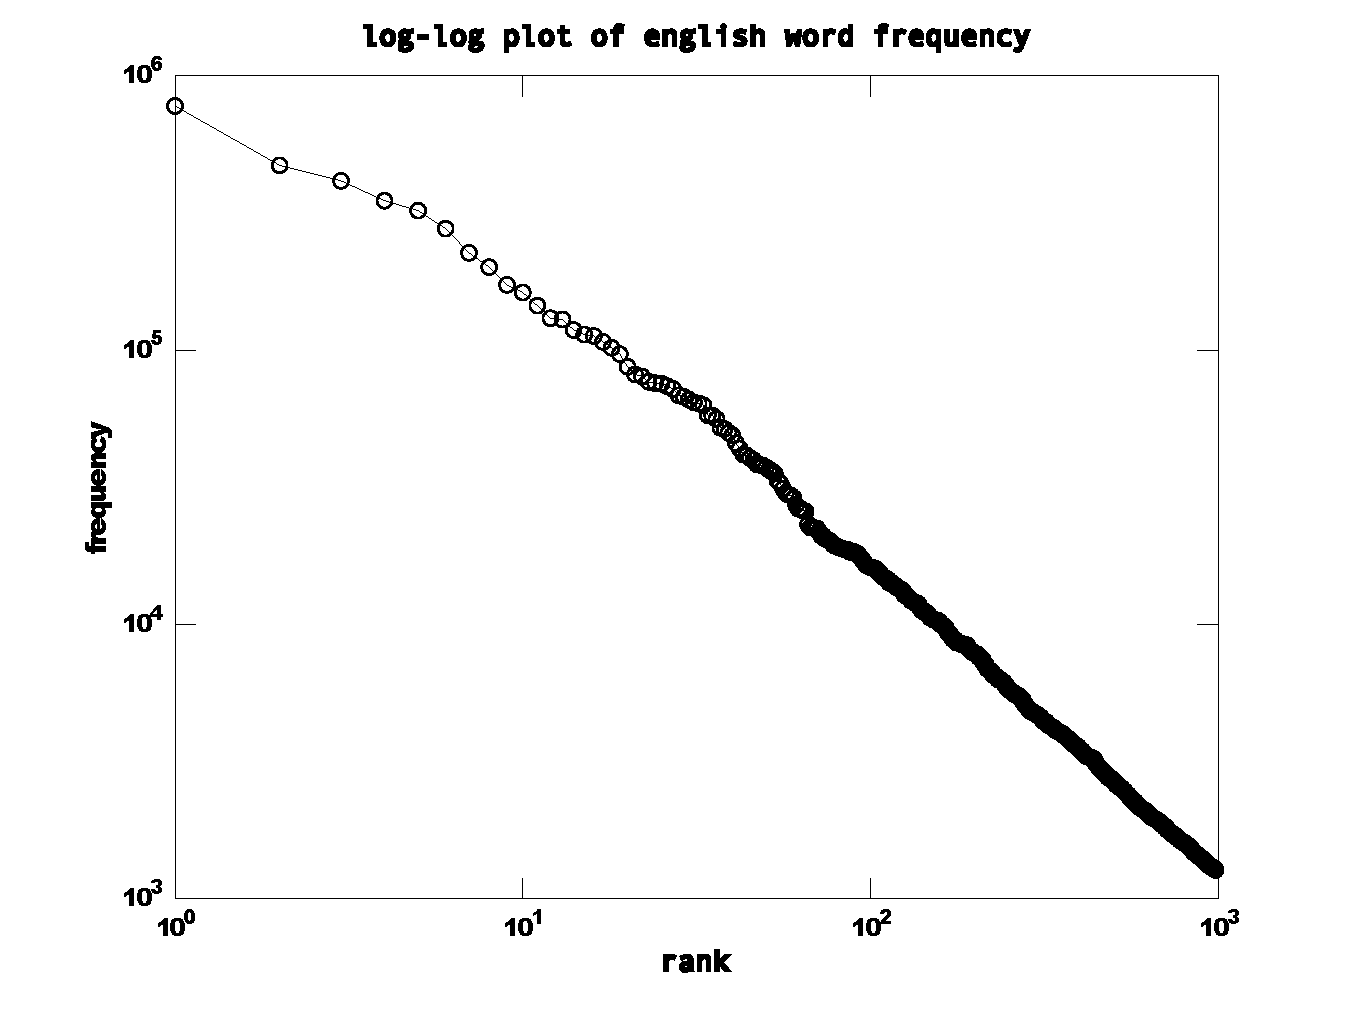
\includegraphics[width=0.75\textwidth]{images/wordfrequency_en.pdf}
\caption{Log-log plot of words rank versus frequency of occurrence (only the 1,000 first words are presented).}
\label{fig:wordfrequency_en}
\end{figure} 

In the analysis presented, all strings of letters separated by white spaces were considered words. The definition of word itself is, in certain aspects, dubious. It is considered as the smallest free form that can be uttered or written and carries a meaning. This is the concept introduced by \cite{bloomfield1926} but it is doubtful since some words are not minimal free forms, like \textit{the} and \textit{of}, which make no meaning by themselves. There are also those meanings that require two strings of letters to express themselves, like: \textit{stock market}, \textit{apple tree}, \textit{carbon dioxide}, \textit{electric guitar}, \textit{hot tub}, \textit{cotton candy}, \textit{dental floss}, \textit{hot dog}, among others. There are some words that are clearly compound ones, like: \textit{newspaper}, \textit{thumbnail}, \textit{copperhead}, \textit{eyelid}, \textit{bedroom}, etc.; and from the previous example, we see that there is a tendency of some two words becoming a compound word, for example, \textit{hot dog} it also written as \textit{hotdog}. In other languages, like German, it is even harder to settle the boundaries of words. In 1996, the German word \textit{Donaudampf\-schifffahrt\-selektrizitäten\-haupt\-betriebs\-werkbau\-unter\-beamten\-gesellschaft} (Association for subordinate officials of the head office management of the Danube steamboat electrical services) was added to the Guinness Book of World Records as the largest word in that language. But the longest word that is not created artificially seems to be \textit{Rindfleische\-tikettierungs\-über\-wachungs\-aufgaben\-über\-tragungs\-gesetz} (Cattle marking and beef labeling supervision duties delegation law).

Anyway, we are interested in language as a spoken means of communication, not a written one, 
although it is known that one influence the other. %(see section \ref{speech_written_interactions}). 
However we don't have a speech database and it would be hard and time consuming to create one, 
we adopted the Carnegie Mellon University (CMU) Pronouncing Dictionary to get the phonetic transcription 
of the words in our database. The CMU Dictionary is a public domain pronouncing dictionary for 
North American English that contains over 125,000 words and their transcriptions. 
It is used as the American lexicon for the Festival Speech Synthesis System and also for 
the CMU Sphinx speech recognition system. Our database extracted from the Gutenberg's books is 
made of 164,444 words (types) and 14,285,332 occurrences of such words (tokens). 
It is still small when compared to the number of entries of some American English dictionaries 
(Merriam-Webster has more than 470,000 entries), but it suffices for a first analysis. 
Unfortunately only 25\% of the words matched the words in the CMU Dictionary, 
some of them because of spelling differences, like the one in \textit{colour - color}, 
\textit{favour - favor} and \textit{neighbourhood - neighborhood}; 
other because they are old-English words, like \textit{thyself}, \textit{milady}, 
\textit{beheld} and \textit{picot}; and all the rest is attributed to misspelling, 
proper names, abbreviations, foreign words or even words that are really not part of 
the CMU Dictionary vocabulary.
% 119,026 out CMU
% 46,094 in CMU

Using the database, transcribed through the CMU Dictionary, it was possible to draw 
some conclusions from the phones usage in English. We present first the list of phones 
and their frequency of occurrence:
\begin{tiny}
\begin{multicols}{4}
\begin{enumerate}
    \item \textipa{@} : 44539 
	\item \textipa{t} : 33131 
	\item \textipa{n} : 31928 
	\item \textipa{I} : 28845 
	\item \textipa{s} : 21928 
	\item \textipa{d} : 20032 
	\item \textipa{r} : 18563 
	\item \textipa{i} : 16482 
	\item \textipa{l} : 15816 
	\item \textipa{E} : 13896 
	\item \textipa{m} : 13072 
	\item \textipa{3\textrhoticity} : 12640 
	\item \textipa{k} : 12308 
	\item \textipa{w} : 11107 
	\item \textipa{z} : 10744 
	\item \textipa{D} : 10720 
	\item \textipa{v} : 10407 
	\item \textipa{h} : 10009 
	\item \textipa{f} : 9391 
	\item \textipa{A} : 8744 
	\item \textipa{\ae} : 8635 
	\item \textipa{b} : 8390 
	\item \textipa{u} : 7972 
	\item \textipa{p} : 7501 
	\item \textipa{O} : 7429 
	\item \textipa{eI} : 6196 
	\item \textipa{aI} : 6148 
	\item \textipa{oW} : 5283 
	\item \textipa{S} : 4915 
	\item \textipa{N} : 4861 
	\item \textipa{g} : 3351 
	\item \textipa{tS} : 2501 
	\item \textipa{j} : 2462 
	\item \textipa{T} : 2309 
	\item \textipa{U} : 2276 
	\item \textipa{aU} : 2242 
	\item \textipa{dZ} : 2100 
	\item \textipa{OI} : 326 
	\item \textipa{Z} : 314 
\end{enumerate}
\end{multicols}
\end{tiny}
The data above are used to plot the frequency of occurrence of the phones against 
their rank, as seen in Figure \ref{fig:phonesfrequency_en}, shown in a log-log plot. 
We may observe that the data don't form a straight line, 
what could be expected, since we are dealing with a very small set and Zipf's law is
characteristic of a class of Large Number of Rare Events (LNRE) \citep{baayen2001}. 
%When we have a set holding a large number of low-probability elements, we expect to
%observe a proportional undersampled subset in any given sample.
Since the number of distinctive phones is quite small, we will observe a reasonably
well estimated phones' probabilities. As we move forward to larger units: bigrams, trigrams,
etc., we expect to increase the chances of observing a power law relation.

%%and we might conclude that they don't follow a Zipf's law-like curve. 
%As already pointed out by \cite{li1992}, ``Zipf's law is not a deep law in natural language 
%as one might first have thought. It is very much related to the particular representation one 
%chooses, i.e., rank as the independent variable.'' \cite{li1992} showed that random texts also 
%exhibit Zipf's law-like curves. 
\cite{li1992} argues that the pattern observed in Zipf's law has significant value
since it is a natural observation on random processes.
Even though, we observe that, as we analyze larger chunks of 
symbols, the relation between the frequency of occurrence of these chunks and their rank 
approximate progressively a Zipf's law (see Figure \ref{fig:simulate_chunks}).

\begin{figure}[h!]
\centering
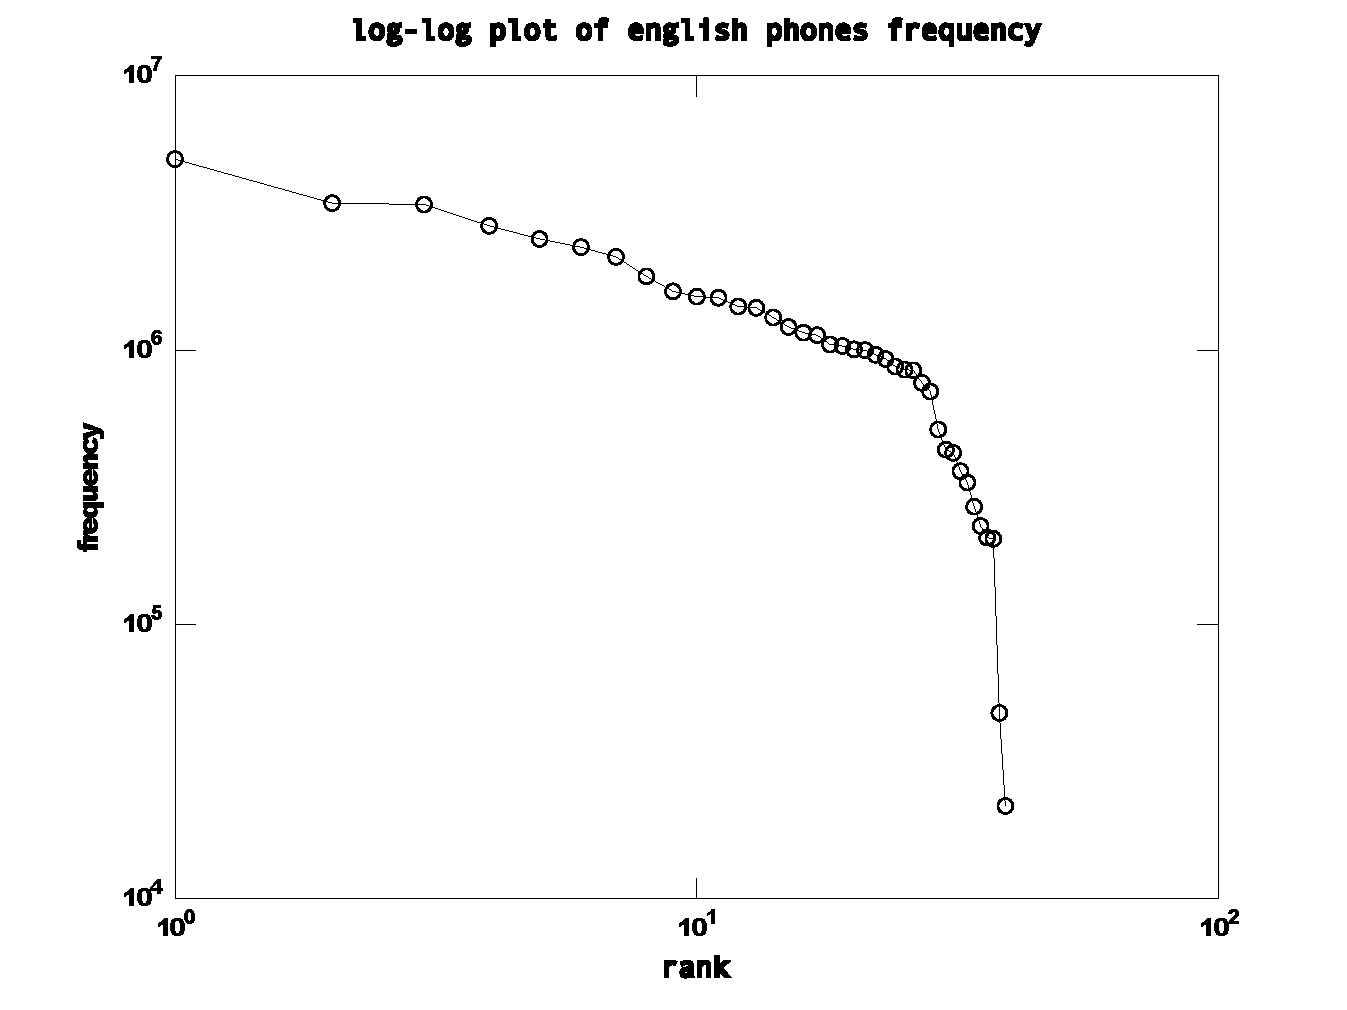
\includegraphics[width=0.75\textwidth]{images/phonesfrequency_en.pdf}
\caption{Log-log plot of phones rank versus frequency of occurrence.}
\label{fig:phonesfrequency_en}
\end{figure} 


\begin{figure}[h!]
%\centering
\noindent\makebox[\textwidth]{%
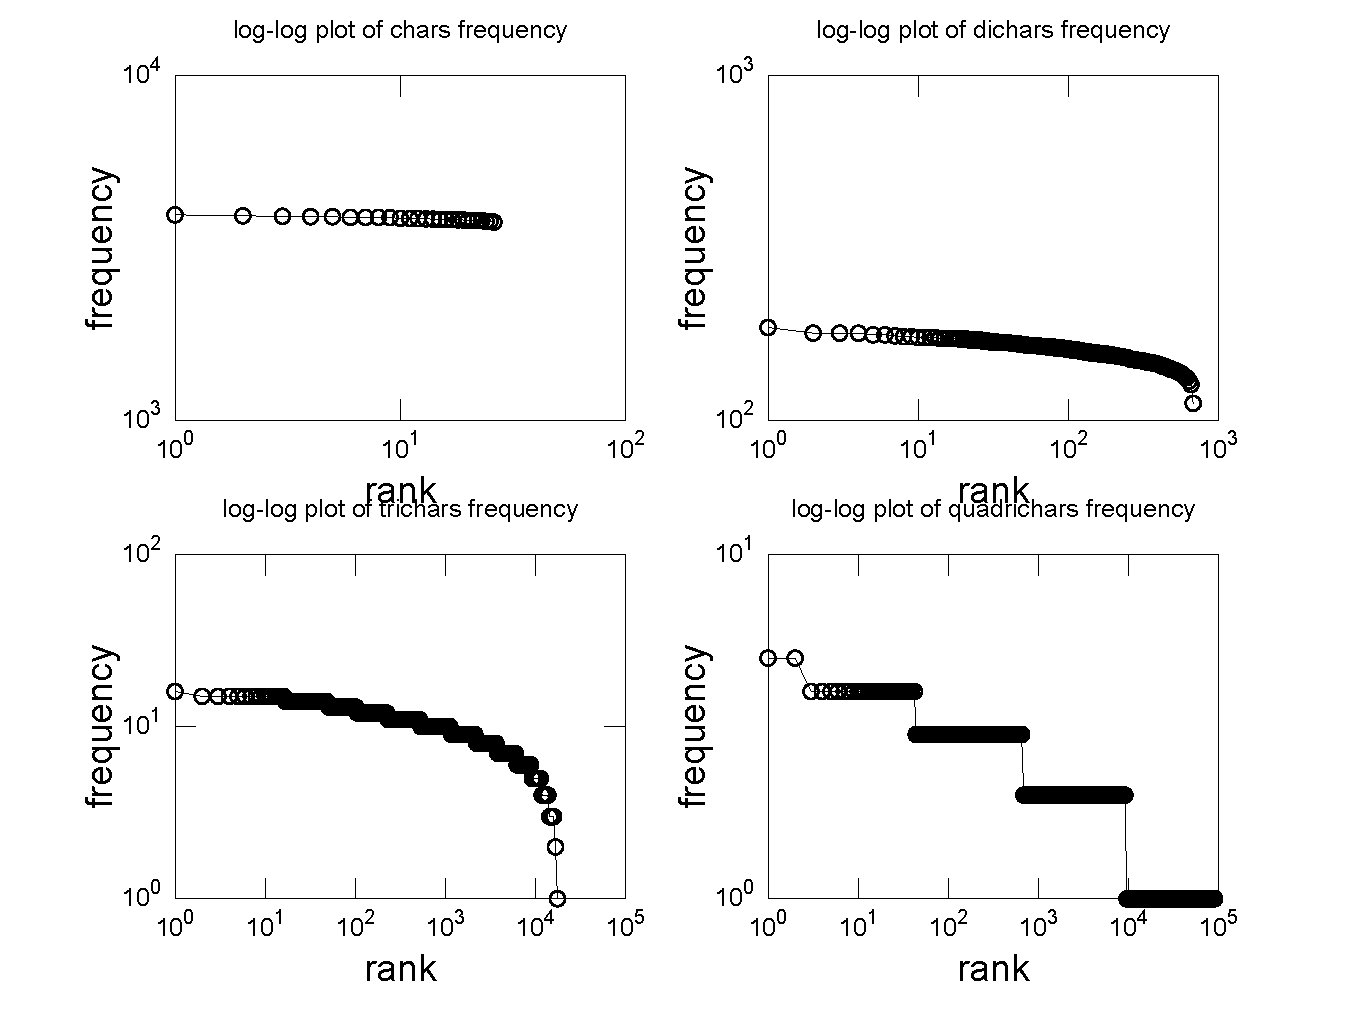
\includegraphics[width=1.0\textwidth]{images/simulate_chunks.pdf} }
\caption{Log-log plot of the rank of chunks of different sizes versus their frequency of occurrence.}
\label{fig:simulate_chunks}
\end{figure}

Another way to see the Zipf's law is as a distribution of Pareto. The Pareto principle states that, for many events, most of the effects come from the minority of the causes.  This principle was named after the Italian economist Vilfredo Pareto. In 1906, he observed that 80\% of the land in Italy was owned by 20\% of the population. The phrase ``The $k$th most frequent word has $n$ occurrences'' may be stated, from the Pareto's perspective, as ``$k$ words occur $n$ or more times''. A Pareto plot is shown in Figure \ref{fig:phones_pareto}. It combines a bar chart displaying percentages of the English phones (categories) with a line graph showing cumulative percentages of these categories. We observe that the 8 first most frequent phones (\textipa{[@, t, n, s, I, r, d, l]}) account for half of all phones occurrences in the data. 
In turn, the Figure \ref{fig:phonesfrequencyocc_en} is a simple ordinary plot of the phones and their respective frequency of occurrence. 
%The last figure \ref{fig:phonescumulativeprobability_en} presents the cumulative distribution for the English phones. 


\begin{figure}[h!]
%\centering
\noindent\makebox[\textwidth]{%
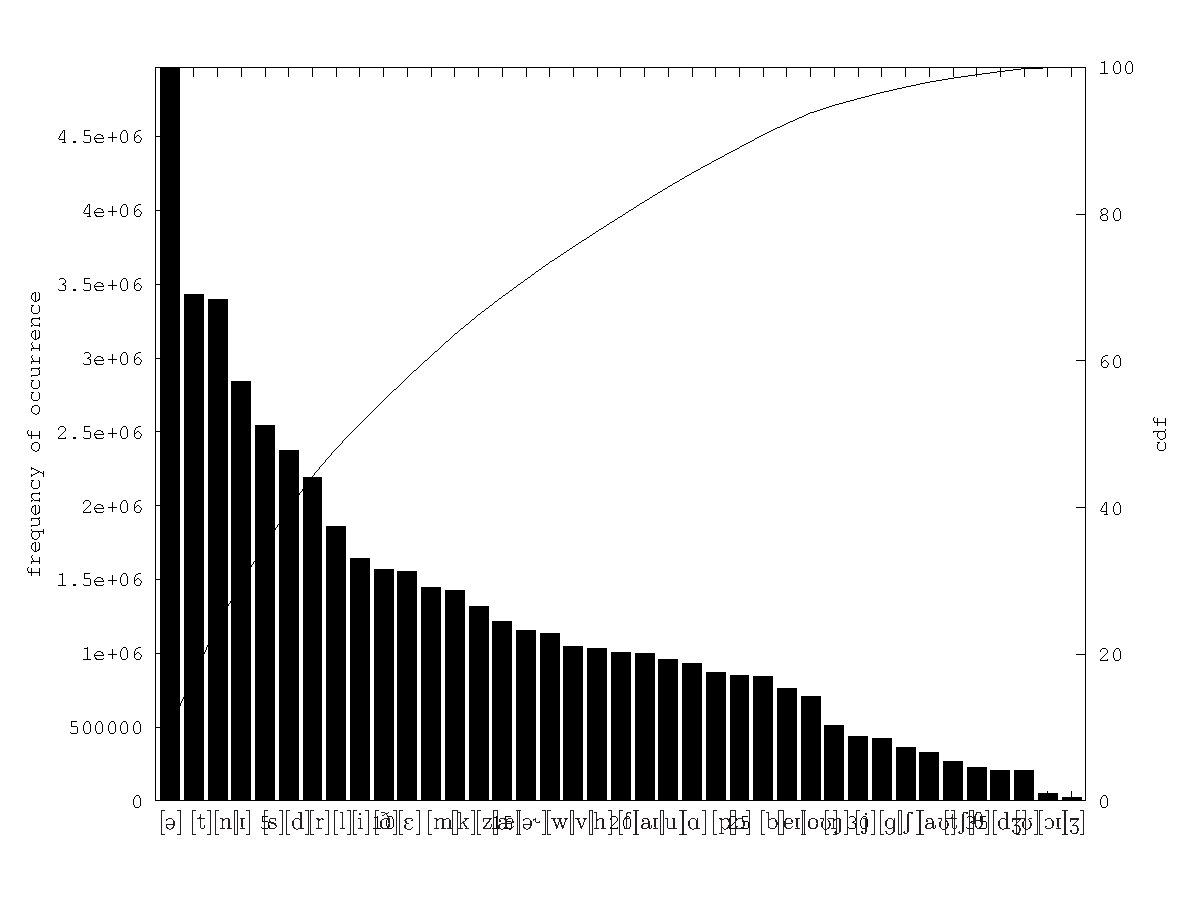
\includegraphics[width=0.95\textwidth]{images/phones_pareto.pdf}
}
\caption{Pareto plot of the English phones.}
\label{fig:phones_pareto}
\end{figure} 





\begin{figure}[h!]
%\centering
\noindent\makebox[\textwidth]{%
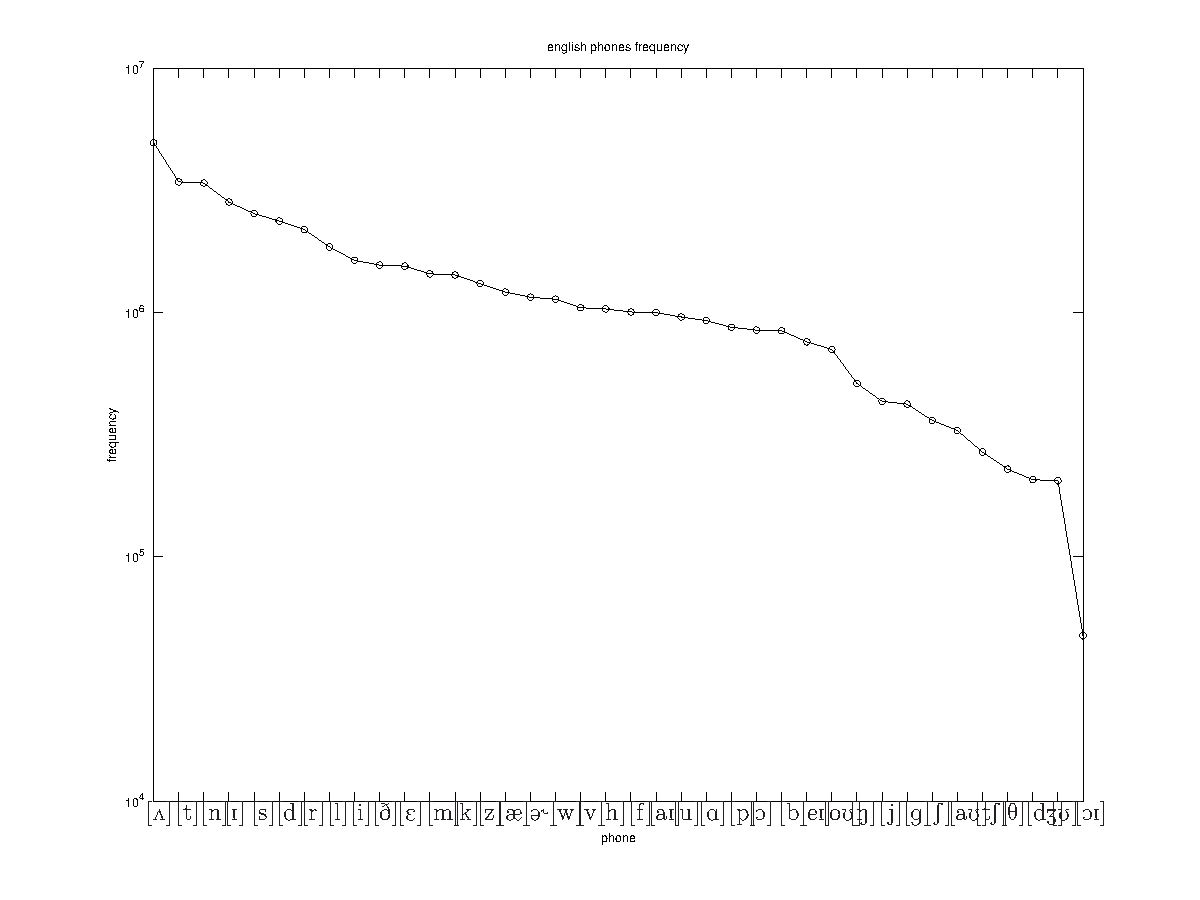
\includegraphics[width=0.95\textwidth]{images/phonesfrequencyocc_en.pdf}
}
\caption{Frequency of occurrence of English phones.}
\label{fig:phonesfrequencyocc_en}
\end{figure} 

%\begin{figure}[h!]
%\centering
%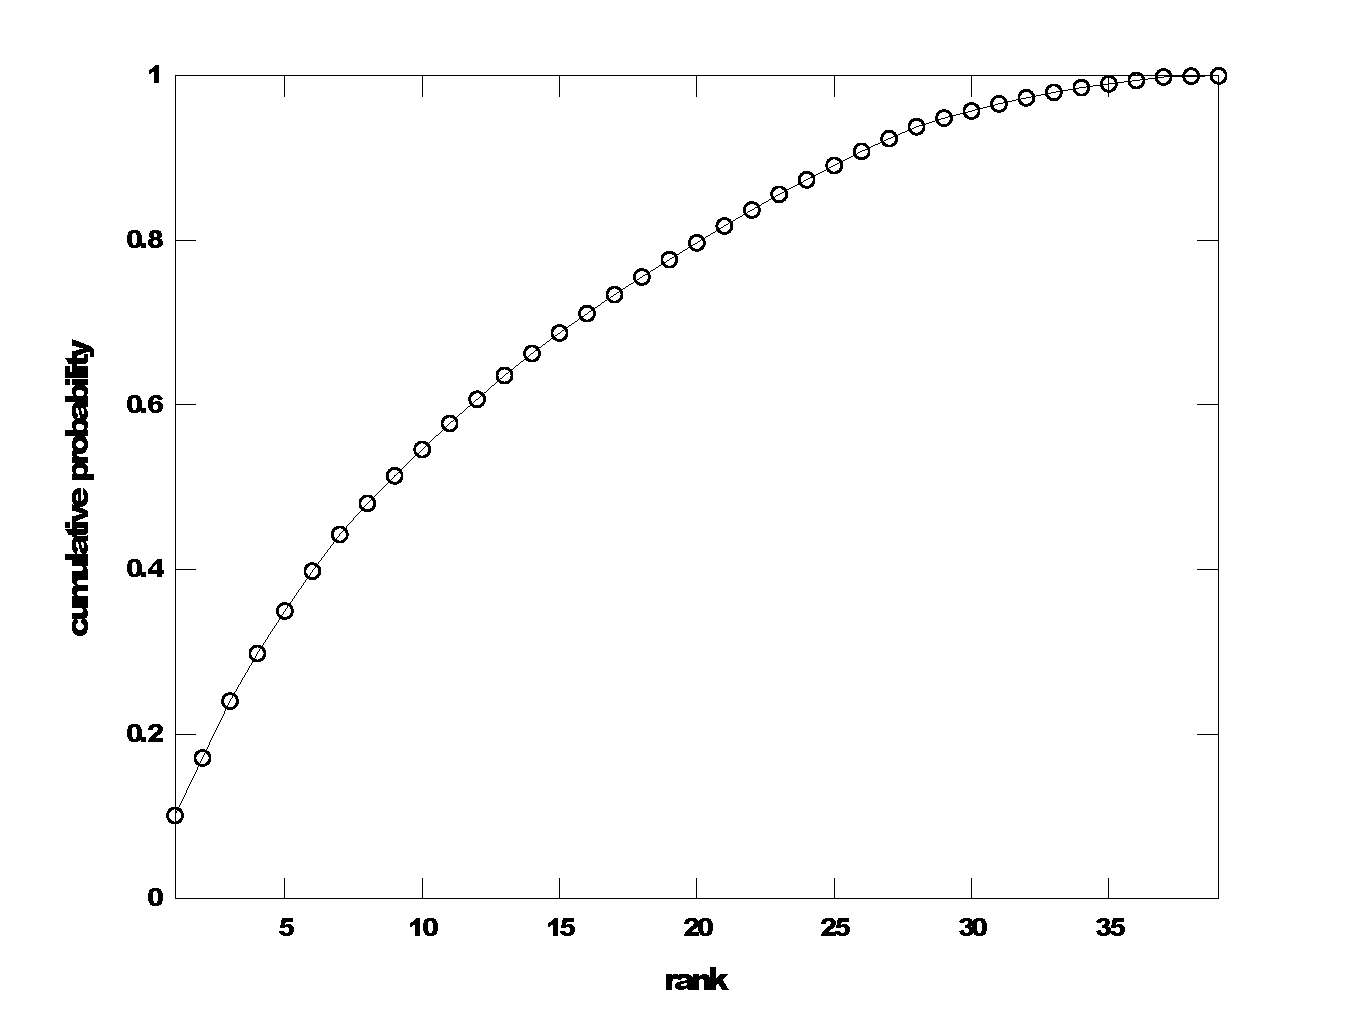
\includegraphics[width=0.75\textwidth]{images/phonescumulativeprobability_en.pdf}
%\caption{Frequency of occurrence of English phones.}
%\label{fig:phonescumulativeprobability_en}
%\end{figure} 


%%%% mover este paragrafo para outro lugar!!!
One important quantity that might be obtained from a database is a measure of the information
being transmitted by a source using a given set of symbols. The notion of information
is dealt by the concept of entropy (what be will discussed in more details in another section)
and is usually measured in bits. The greater the entropy of a source, the greater is the 
uncertainty associated with its output and then it is also greater the amount of information encoded
in its messages.
The entropy of spoken English, calculated from the data above, gives 4.84 bits per phone.
%which is considerably higher compared to the entropy of written English,
The entropy of written English was estimated by \citep{schneier1996}, who found it
to be between 1.0 and 1.5 bits per letter. %\citep{schneier1996}, 
It was also estimated by \cite{shannon1951}, having found a value between 0.6 and 1.3 bits per letter,
%what was found by \cite{shannon1951} 
in a experiment where subjects were asked to predict
the next letter in a English text. 
The relative entropy, Kullback–Leibler divergence, of English 
phones compared to a uniform random distribution is 0.45 bits.
%0.48 bits.

Zipf believed that the change in frequency was responsible for triggering the 
mechanism of combination. He supposes that the frequency of occurrence of a
lower level unity is proportional to the number of higher level structures 
it will appear on. The low specificity of a lower level unit
makes it more suitable for been used in making higher level structures.
Figure \ref{fig:phones_num_words_freq_occ} presents the relationship
between the frequency of occurrence of English phones and the number
of English words they appear on. 

\begin{figure}[h!]
\centering
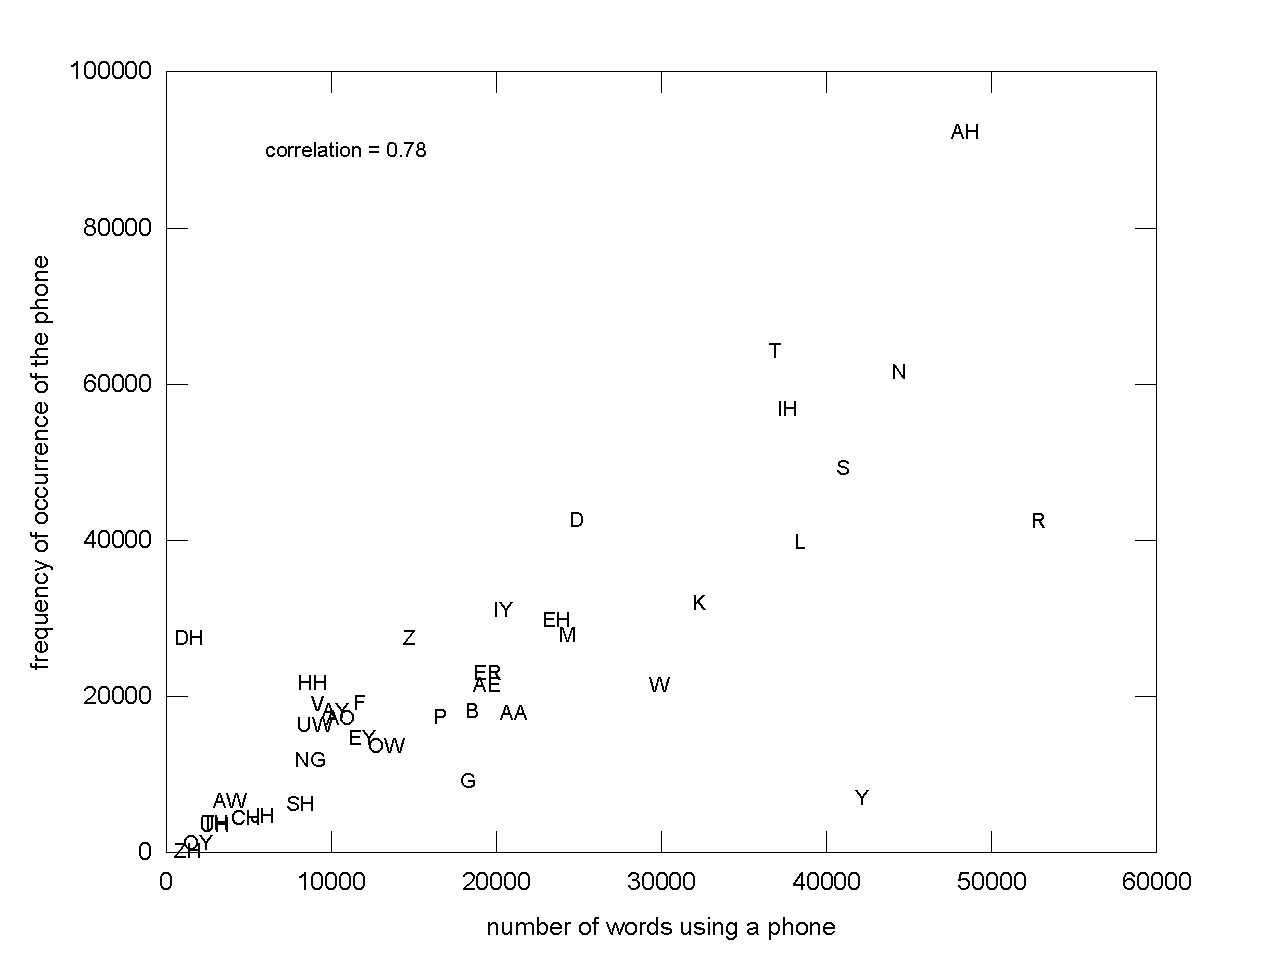
\includegraphics[width=0.65\textwidth]{images/phones_num_words_freq_occ.pdf}
\caption{Relation between the frequency of occurrence of phones and the number of words they appear.}
\label{fig:phones_num_words_freq_occ}
\end{figure} 

The distribution of the occurrence of a given phone is not uniform across the rank of words in a language. 
Nor can't we conclude that the high frequency of certain phones is due to the high frequency of the words they appear. 
Figure \ref{fig:proboccwordsphone} shows the probability of occurrence of phones across the rank of words. 
We might observe that the probability of occurrence of a given phone is greater in rare words then in usual ones.
%against what we could intuitively conclude without an analysis of the data.
Since high rank words are longer, the probability of occurring any phone is greater than on low rank words.

\begin{figure*}[p]
  \centering 
  %\captionsetup[subfigure]{margin=10pt,singlelinecheck=false}
  \begin{tabular}{cc}
  \subfloat[Probability of occurrence of \textipa{[@]} in words versus words rank.]{\label{fig:proboccwordsphone_AH}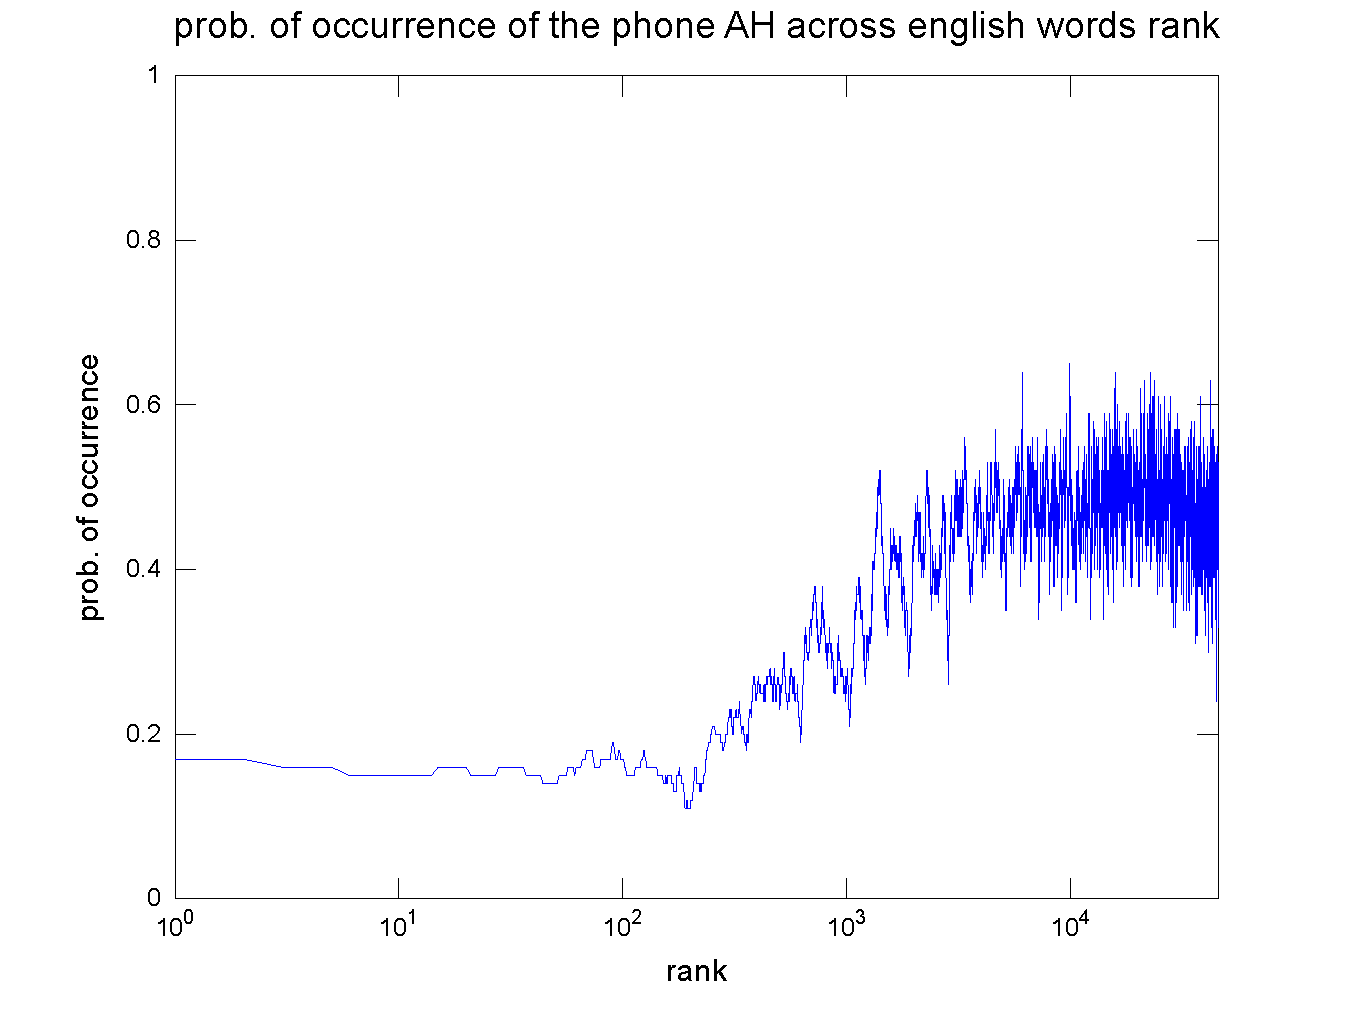
\includegraphics[width=0.45\textwidth]{images/proboccwordsphone_AH.pdf}} &
  \subfloat[Probability of occurrence of \textipa{[t]} in words versus words rank.]{\label{fig:proboccwordsphone_T}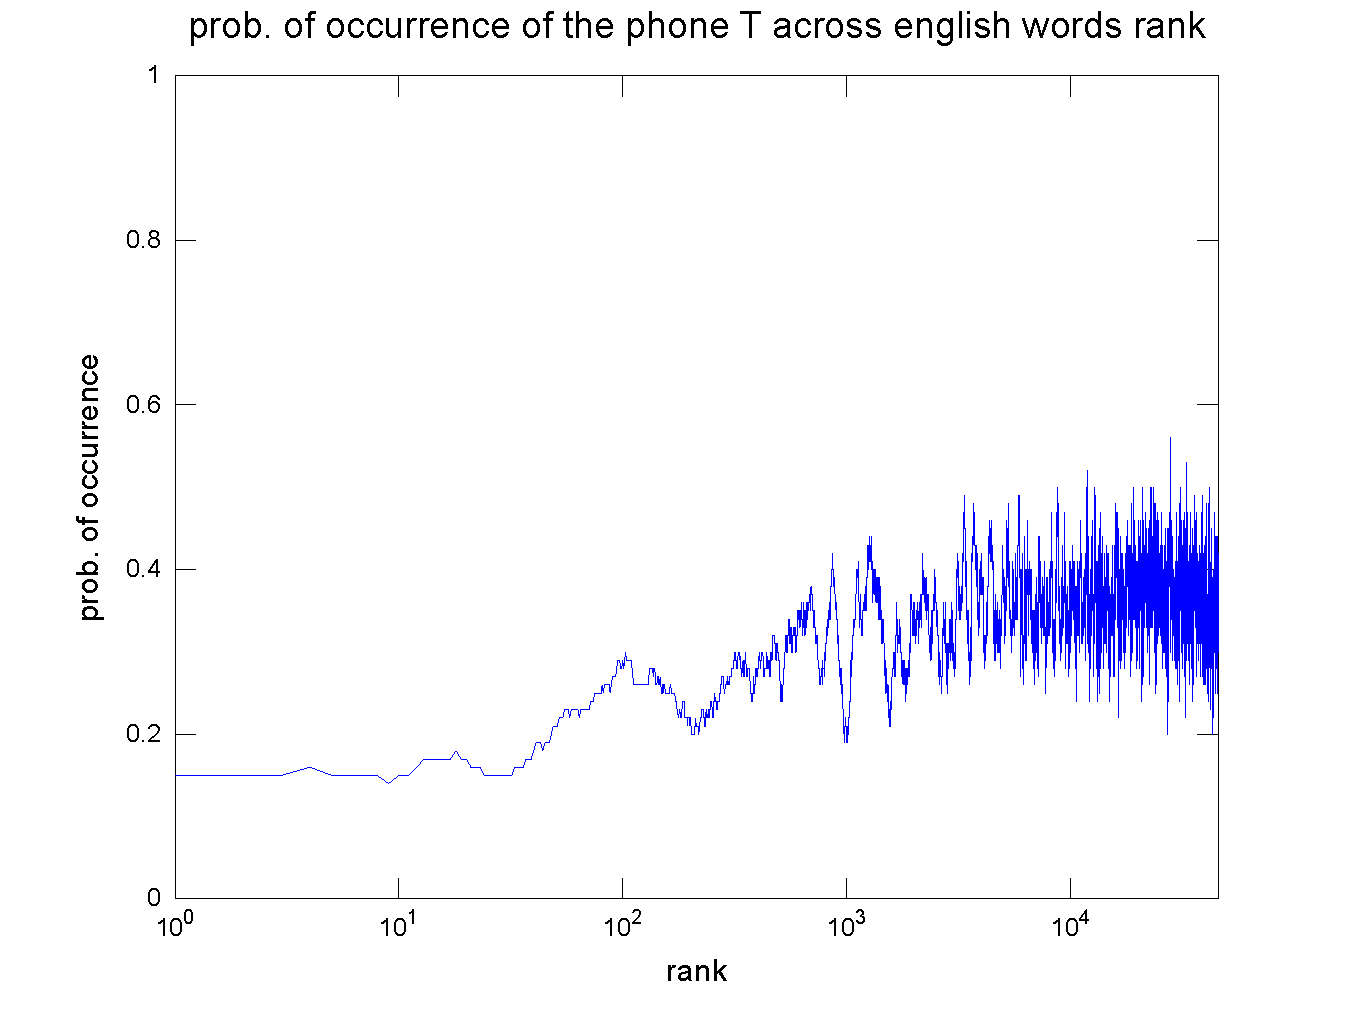
\includegraphics[width=0.45\textwidth]{images/proboccwordsphone_T.pdf}} \\
  \subfloat[Probability of occurrence of \textipa{[n]} in words versus words rank.]{\label{fig:proboccwordsphone_N}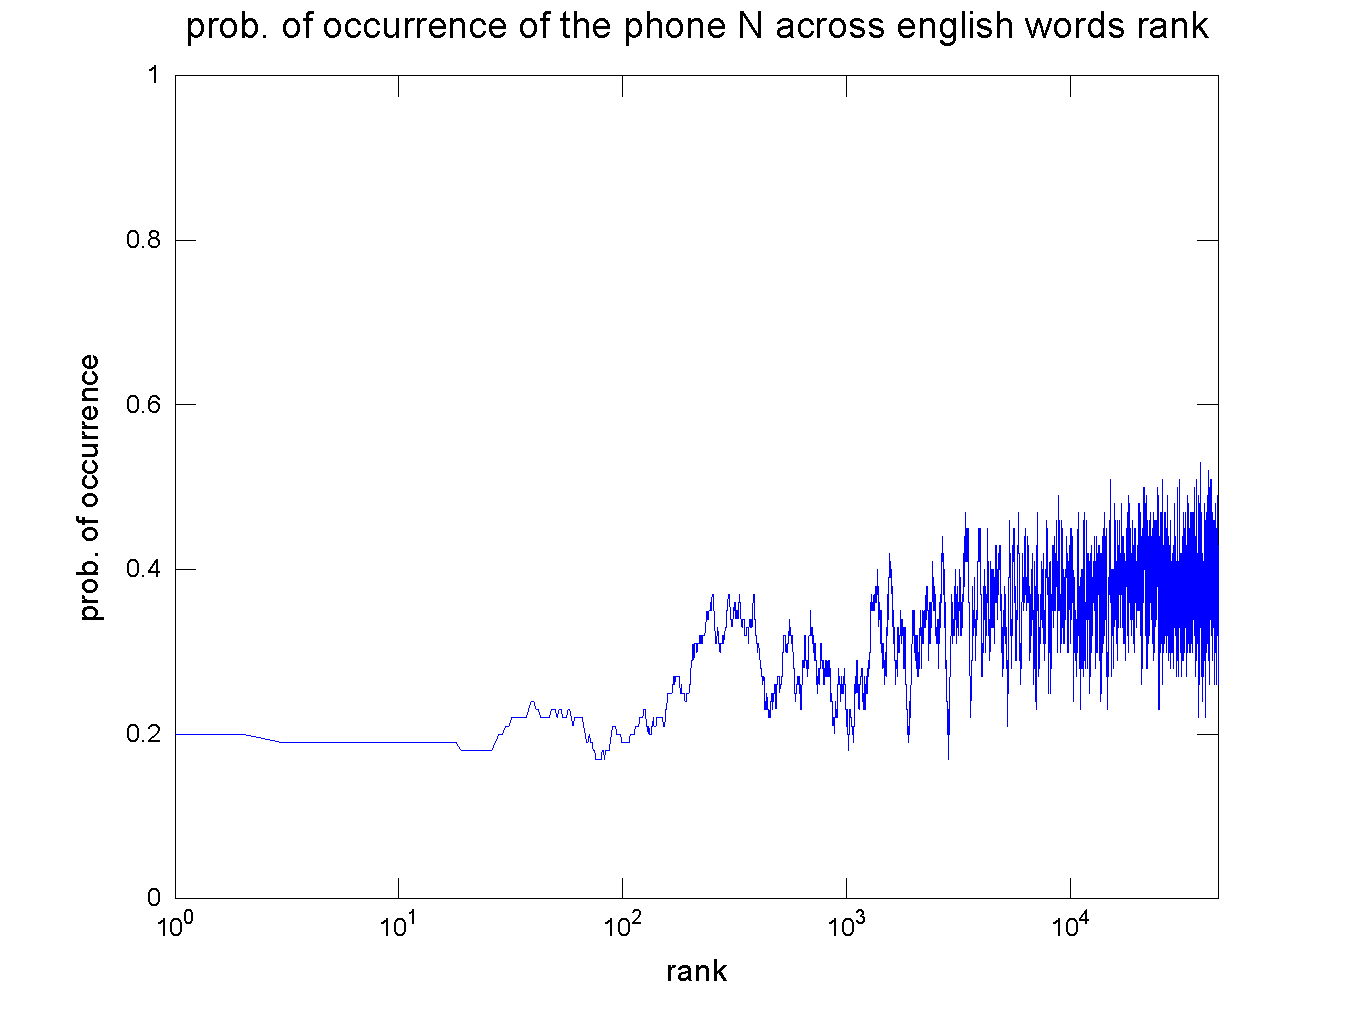
\includegraphics[width=0.45\textwidth]{images/proboccwordsphone_N.pdf}} &
  \subfloat[Probability of occurrence of \textipa{[U]} in words versus words rank.]{\label{fig:proboccwordsphone_UH}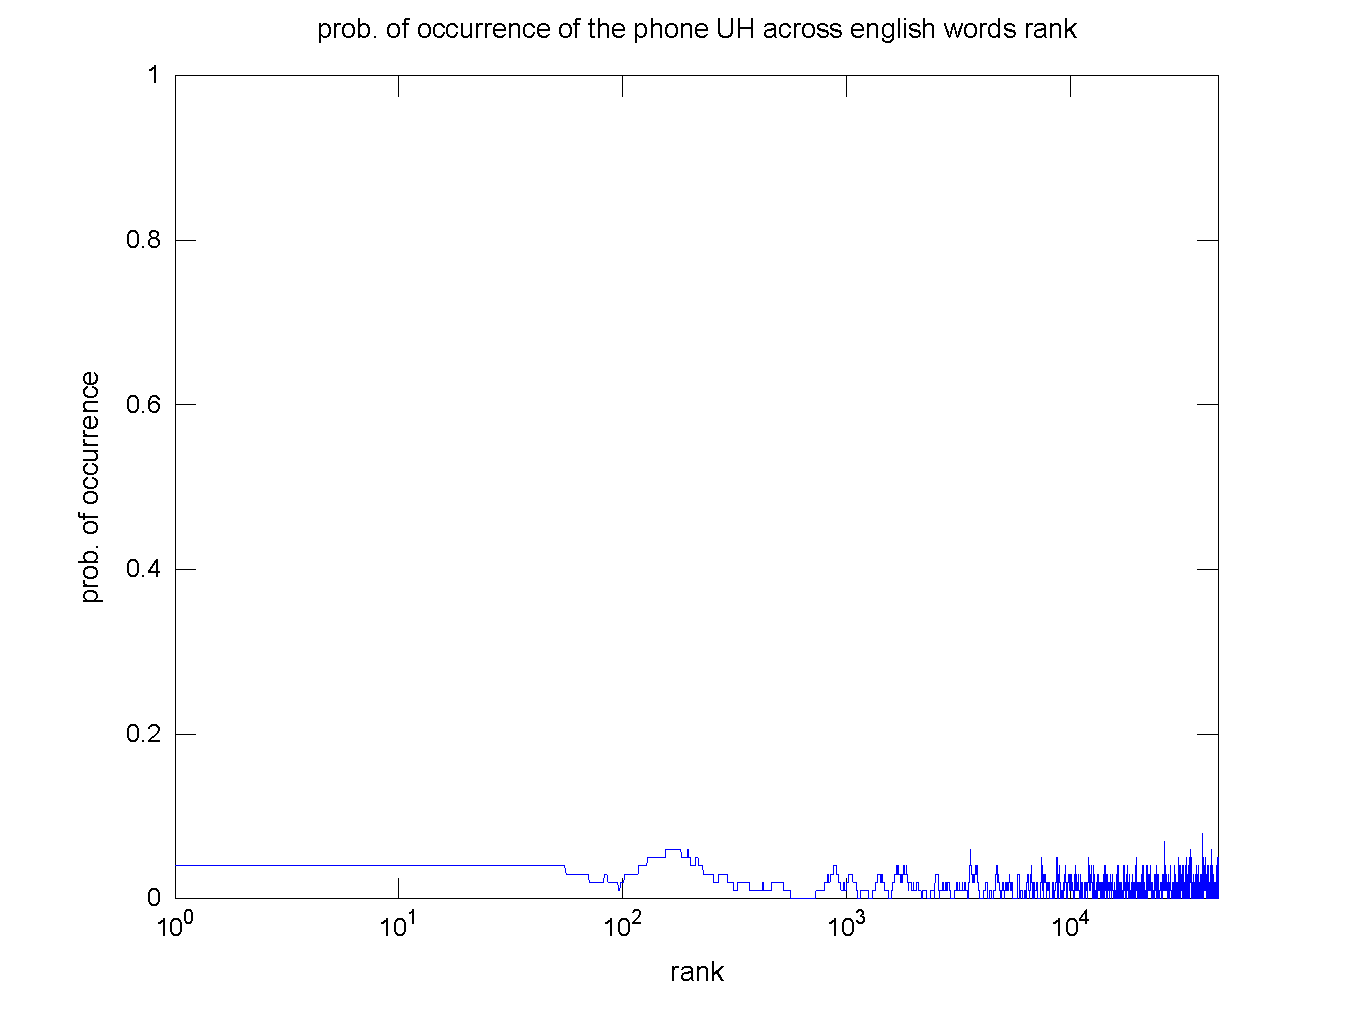
\includegraphics[width=0.45\textwidth]{images/proboccwordsphone_UH.pdf}} \\
  \subfloat[Probability of occurrence of \textipa{[OI]} in words versus words rank.]{\label{fig:proboccwordsphone_OY}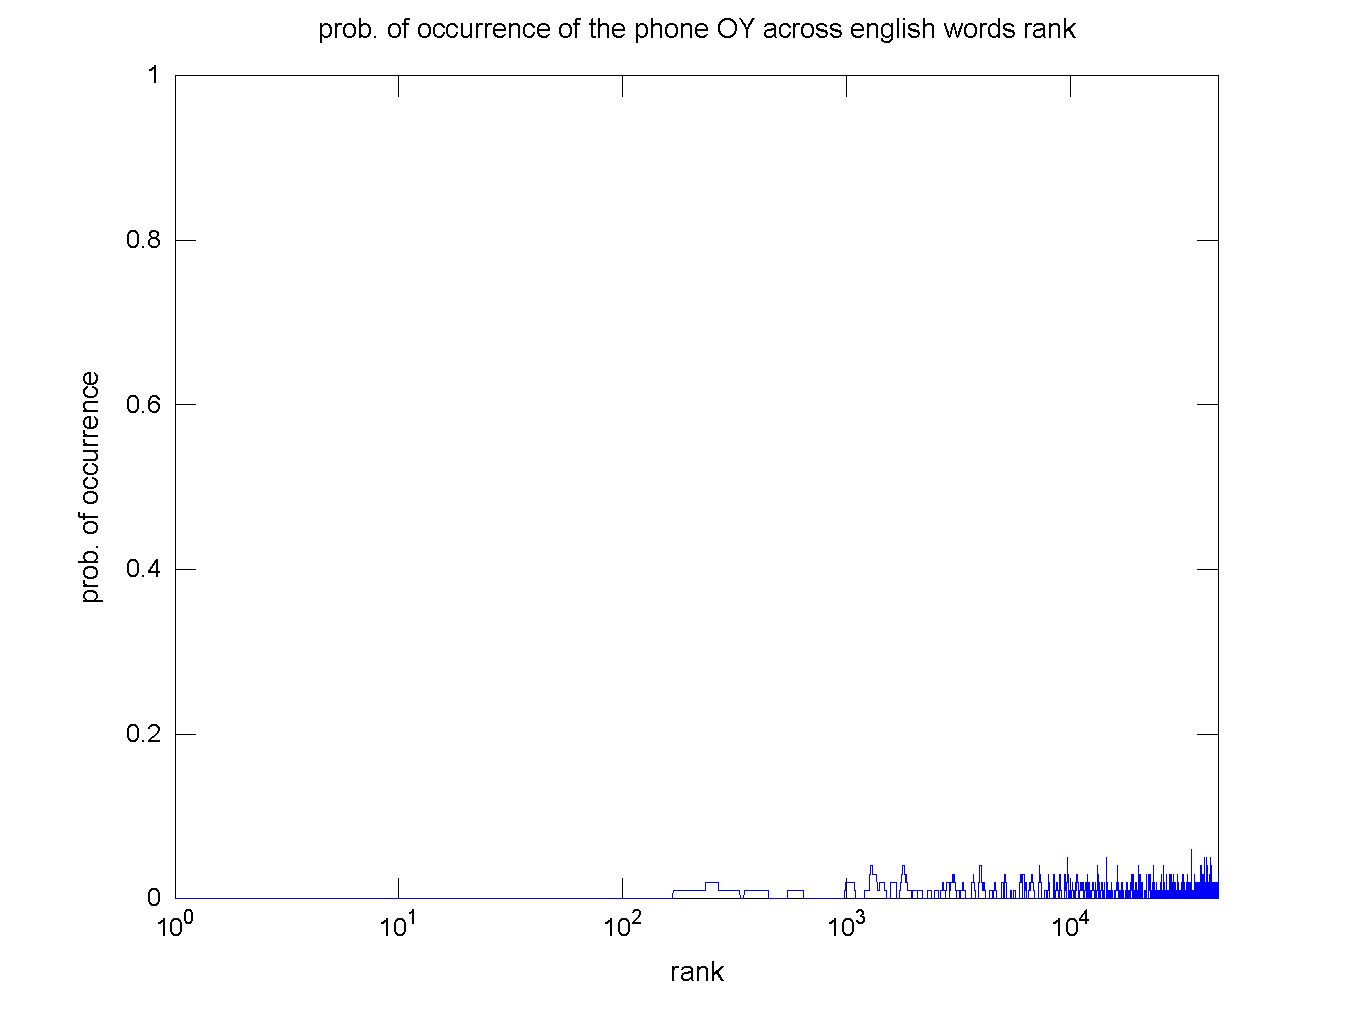
\includegraphics[width=0.45\textwidth]{images/proboccwordsphone_OY.pdf}} & 
  \subfloat[Probability of occurrence of \textipa{[Z]} in words versus words rank.]{\label{fig:proboccwordsphone_ZH}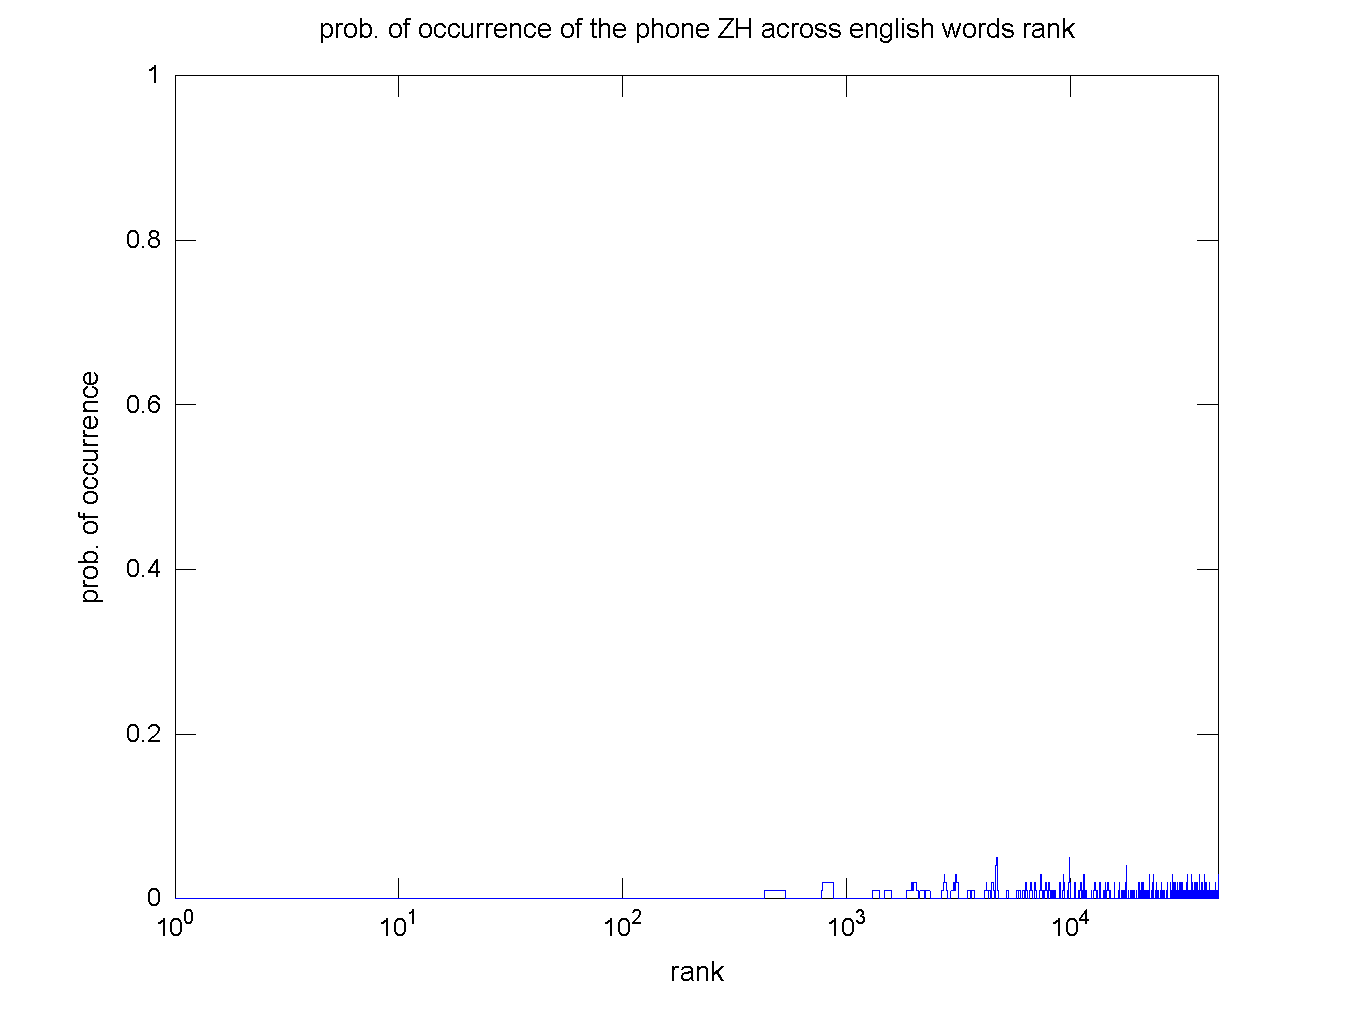
\includegraphics[width=0.45\textwidth]{images/proboccwordsphone_ZH.pdf}} 
  \end{tabular}
  \caption{Probability of occurrence of certain phones in words across the rank of words.}
  \label{fig:proboccwordsphone}
\end{figure*}

Analyzing the sound systems of human languages, we conclude that they show remarkable regularities. Although humans are able to pronounce and perceive a great variety of speech sounds, languages use only a subset of them. Under another perspective, the categories created by languages, in order to achieve communication, form a small subset of possible categories of speech sounds that have a certain regularity across languages. Those regularities might be explained by innate human cognitive capacities or by functional constraints of communication. Such constraints would be created by the requirement of language to be a robust learnable means of communication, which would be responsible for the existence of redundancy, predictability, distinguishability and the usage of sounds of easy understandability and repeatability.

In the analysis of 451 languages of the world made by \cite{maddieson1884} using the UPSID (the UCLA Phonological Segment Inventory Database), 921 different speech sounds are found. As shown in Figure \ref{fig:language_segments_hist}, most of the languages (66.3\%) have a repertoire of 20 to 37 speech sounds. 
%The maximal number of elements used is 141 in !X\~u; and the minimal is 11 in Rotokas and Pirah\~a. 
%That means, 
In each language, we use only a subset of all the speech sounds available (using as a reference the UPSID and the 919 phones on this database, 
a language typical uses between 1.2\% and 15.3\% of the available speech sounds). Analyzing the subsets used in each language, we present bellow 
a list of the 20 most frequent consonants and the 10 most frequent vowels (see tables \ref{tbl:consonants_most_freq} and \ref{tbl:vowels_most_freq}).


\begin{table}[h]
\caption{List of the 20 most frequent consonants in UPSID.}
\label{tbl:consonants_most_freq}
\begin{tabular}{|c|c|c|c|c|c|c|c|c|}
\hline consonant 		& \textipa{m} & \textipa{k} & \textipa{j} & \textipa{p} & \textipa{w} & \textipa{b} & \textipa{h} & \textipa{g} \\ 
\hline n. of languages	& 425 & 403 & 378 & 375 & 332 & 287 & 279 & 253 \\ 
\hline frequency 		& 94.2 & 89.4 & 83.8 & 83.2 & 73.6 & 63.6 & 61.9 & 56.1 \\ 
\hline 
\end{tabular} 

\begin{tabular}{|c|c|c|c|c|c|c|c|c|}
\hline consonant 		& \textipa{N} & \textipa{P} & \textipa{n} & \textipa{s} & \textipa{tS} & \textipa{S} & \textipa{t} & \textipa{f} \\ 
\hline n. of languages	& 237 & 216 & 202 & 196 & 188 & 187 & 181 & 180 \\ 
\hline frequency 		& 52.6 & 47.9 & 44.8 & 43.5 & 41.7 & 41.5 & 40.1 & 39.9 \\ 
\hline 
\end{tabular} 

\begin{tabular}{|c|c|c|c|c|}
\hline consonant 		& \textipa{l} & \textipa{\|[n} & \textipa{\|[t} & \textipa{\textltailn } \\ 
\hline n. of languages	& 174 & 160 & 152 & 141 \\ 
\hline frequency 		& 38.6 & 35.5 & 33.7 & 31.3 \\ 
\hline 
\end{tabular} 
\end{table}


\begin{table}[h]
\caption{List of the 10 most frequent vowels in UPSID.}
\label{tbl:vowels_most_freq}
\begin{tabular}{|c|c|c|c|c|c|c|c|c|c|c|}
\hline consonant 		& \textipa{i} & \textipa{a} & \textipa{u} & \textipa{E} & \textipa{o/O} & \textipa{e/E} & \textipa{O} & \textipa{o} & \textipa{e} & \textipa{~a} \\ 
\hline n. of languages	& 393 & 392 & 369 & 186 & 181 & 169 & 162 & 131 & 124 & 83 \\ 
\hline frequency 		& 87.1 & 86.9 & 81.8 & 41.2 & 40.1 & 37.5 & 35.9 & 29.0 & 27.5 & 18.4 \\ 
\hline 
\end{tabular} 
\end{table}

Comparing tables \ref{tbl:consonants_most_freq} and \ref{tbl:vowels_most_freq}, we observe that the most frequent vowels are not so frequent across languages in comparison to the most frequent consonants. In the UPSID, there are 180 vowels, 16 glides\footnote{Glide or semivowel contrast with vowels by being non-syllabic, they functions as the syllable boundary rather than nucleus. In our analysis we will consider only the following as semivowels: palatal approximant, labial-palatal approximant, velar approximant, labial-velar approximant, and their possible variations.\citep{martinezceldran2004}} and 725 consonants, which strongly outnumber the others. The languages in UPSID present from 6 to 117 consonants (and glides), averaging 22.7 and from 3 to 28 vowels, averaging 8.1. The ratio consonant to vowel ranged from 0.69 to 15.33, averaging about 3.38. On average, languages present three times as many consonants as vowels. Considering that the database with 451 languages has in its inventory 652 consonants and 269 vowels, we see that across the languages, the number of vowels used corresponds from 0.9\% to 17.9\% (averaging 3.0\%) of the possible vowels; and the number of consonants used goes from 0.9\% to 14.6\% (averaging 3.5\%) of the consonants in the database. We might then conclude that the segments are chosen proportionally among all the possibilities, there is no tendency in choosing consonant over vowels, or the other way around. Analyzing these results and those on tables \ref{tbl:consonants_most_freq} and \ref{tbl:vowels_most_freq}, we conclude that there is some sort of stronger constraint on consonants that push some of them to become more frequent across languages. A constraint of this kind also exists for vowels, but it is much weaker. We also observe that, in general, languages use a speech repertoire where the number of consonants is greater than the number of vowels. There are only 14 languages (Kashmiri, Bruu, Dan, Klao, Kaingang, Apinaye, Barasano, Yagua, Cubeo, Japreria, Panare, Andoke, Maxakali, Vanimo) in which the number of vowels is greater or equal to the number of consonants. There are 427 speech sounds that are present in only one language. The group of sounds that appear in 10 or fewer of the 451 languages in the database sum up more that 80\% of all 919 sounds in the database.


%180 vowels
%palatal approximant : 5
%labial-palatal approximant : 1
%velar approximant : 6
%labial-velar approximant : 4

% min(numVowels) =  3
% max(numVowels) =  28
% mean(numVowels) =  8.0532

% min(numConsonants) =  6
% max(numConsonants) = 117
% mean(numConsonants) =  22.663

% ratio = numConsonants./numVowels
% min(ratio) =  0.68750
% max(ratio) =  15.333
% mean(ratio) =  3.3798


Figure \ref{fig:freqidx_nsegs_upsid} presents the relationship observed across languages of the 
usage of frequent or rare segments with the number of segments used in that language. 
In order to do so, a frequency index is proposed by \cite{reetz2010}. 
This index is the average of the segment frequencies of the segments in a language. 
Each segment in the UPSID has a segment frequency that is the number of languages that contain 
a specific segment divided by the number of languages in UPSID. 
Each language has a certain segment-repertoire. The frequency index of a language is calculated 
as the average of the frequency index of all segments in a language repertoire. 
``If a language has only few segments, it is likely that these are rather common in the languages 
in UPSID. On the other hand, a language with many segments will also have many segments that are 
uncommon in the UPSID database''\citep{reetz2010}.

\begin{figure}[h!]
\centering
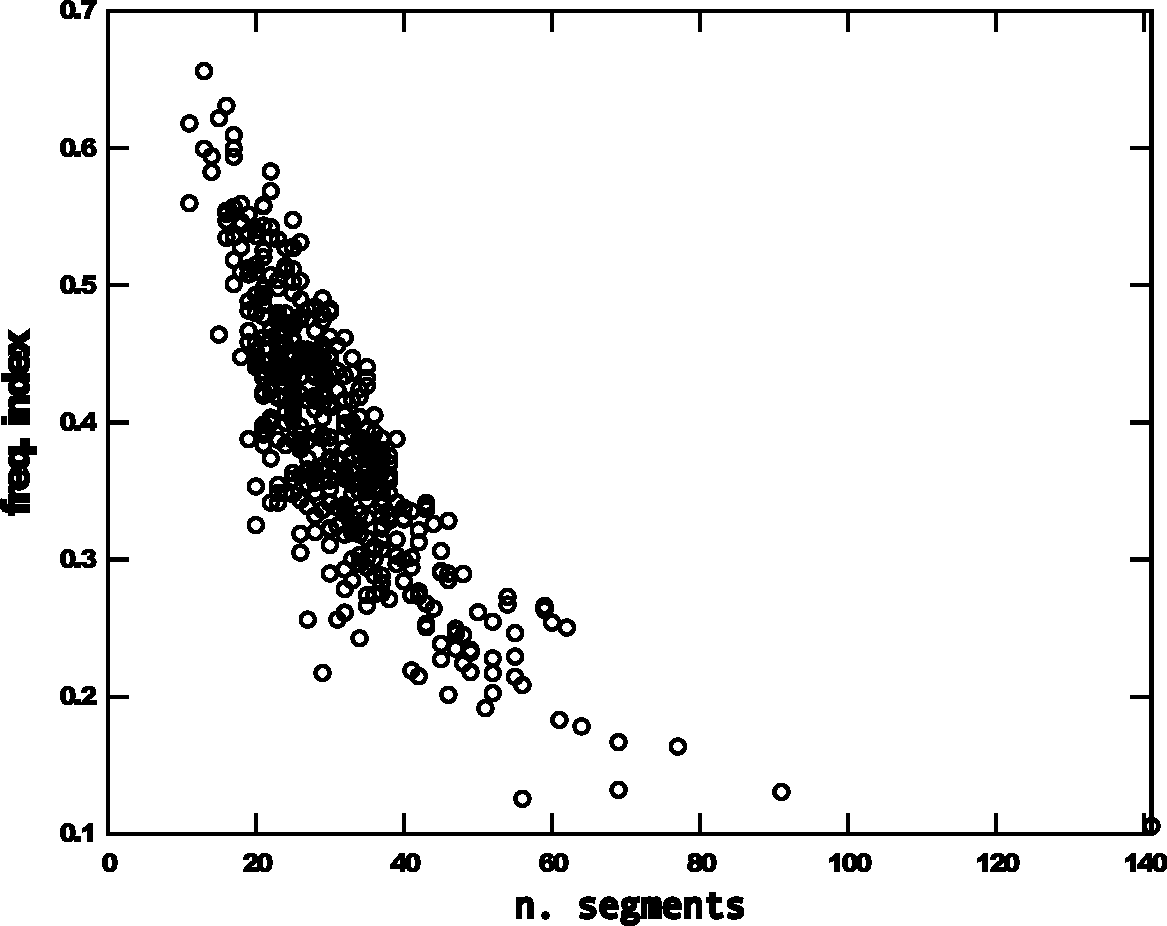
\includegraphics[width=0.65\textwidth]{images/freqidx_nsegs_upsid.pdf}
\caption{Relation between the frequency index and the number of phones in a language. (Data from UPSID)}
\label{fig:freqidx_nsegs_upsid}
\end{figure} 

%To understand how languages are structured, it is also important to 
%observe how categories emerge and how they are used. 
Using the UPSID database, we might find what speech segments co-occurs with each other in
different languages. When addressing the UPSID database, we shall use the term \emph{co-occurrence}  
to make reference to phones that occur in the same inventory. This remark is important in order to avoid
a possible confusion with the usual meaning of \emph{co-occurrence}, that is used to
assign phones that are neighbours in an utterance.  
%At a first glance, we might take on the co-occurrence of speech segments. Using the UPSID database 
We may find what are the most frequent co-occurring segment for another given segment 
(some results are in Figure \ref{fig:cooccurrence} and Table \ref{tbl:cooccurrence}). 
We notice that there is a large number of co-occurring segments for each one taken as a reference. 
The most frequent segments across languages have a great number of co-occurring segments, 
which represent approximately from 30\% to 60\% of all segments in UPSID. On the other hand, 
the most infrequent phones in the database have just a few co-occurring segments, around 3\%. 
Observing the graphics in Figure \ref{fig:cooccurrence}, we see that, for each reference segment, 
the co-occurring ones has a rapidly decreasing frequency of co-occurrence, what is expected from a random distribution. 
The high co-occurrence of certain pairs, in some cases, might be explained by the features they share. 
As an example, if we consider the bilabial consonants, we see that, as we take one as reference, 
the others appear in the top-10 list, showing a strong adhesion of one bilabial consonant to another. 
Observing now the voiced alveolar sibilant fricative \textipa{[z]}, its voiceless counterpart always appear, 
but doing the other way around analysis, taking \textipa{[s]} as a reference, its voiced counterpart \textipa{[z]} 
has a relative frequency of co-occurrence of 31.6\%, figuring as the 29th in the list. 
Analyzing other pairs like \textipa{[t]}-\textipa{[d]}, \textipa{[k]}-\textipa{[g]} and \textipa{[p]}-\textipa{[b]}, 
it seems that the existence of the voiced counterpart subjects the existence of the voiceless much more 
emphatically than the other way around.


\begin{figure*}[p]
  \centering 
  \captionsetup[subfigure]{margin=10pt,singlelinecheck=false,font={scriptsize,sf}}
  \subfloat[This graph presents the co-occurrence frequency for phones in relation to \textipa{[@]}. The phone \textipa{[k]} has a frequency of 96.0\%. \textipa{[m]} follows with 94.7\% and \textipa{[p]} with 90.7\%. 39.8\% of the phones in UPSID are co-occurring with the phone \textipa{[@]}.]{\label{fig:cooccurrence_01}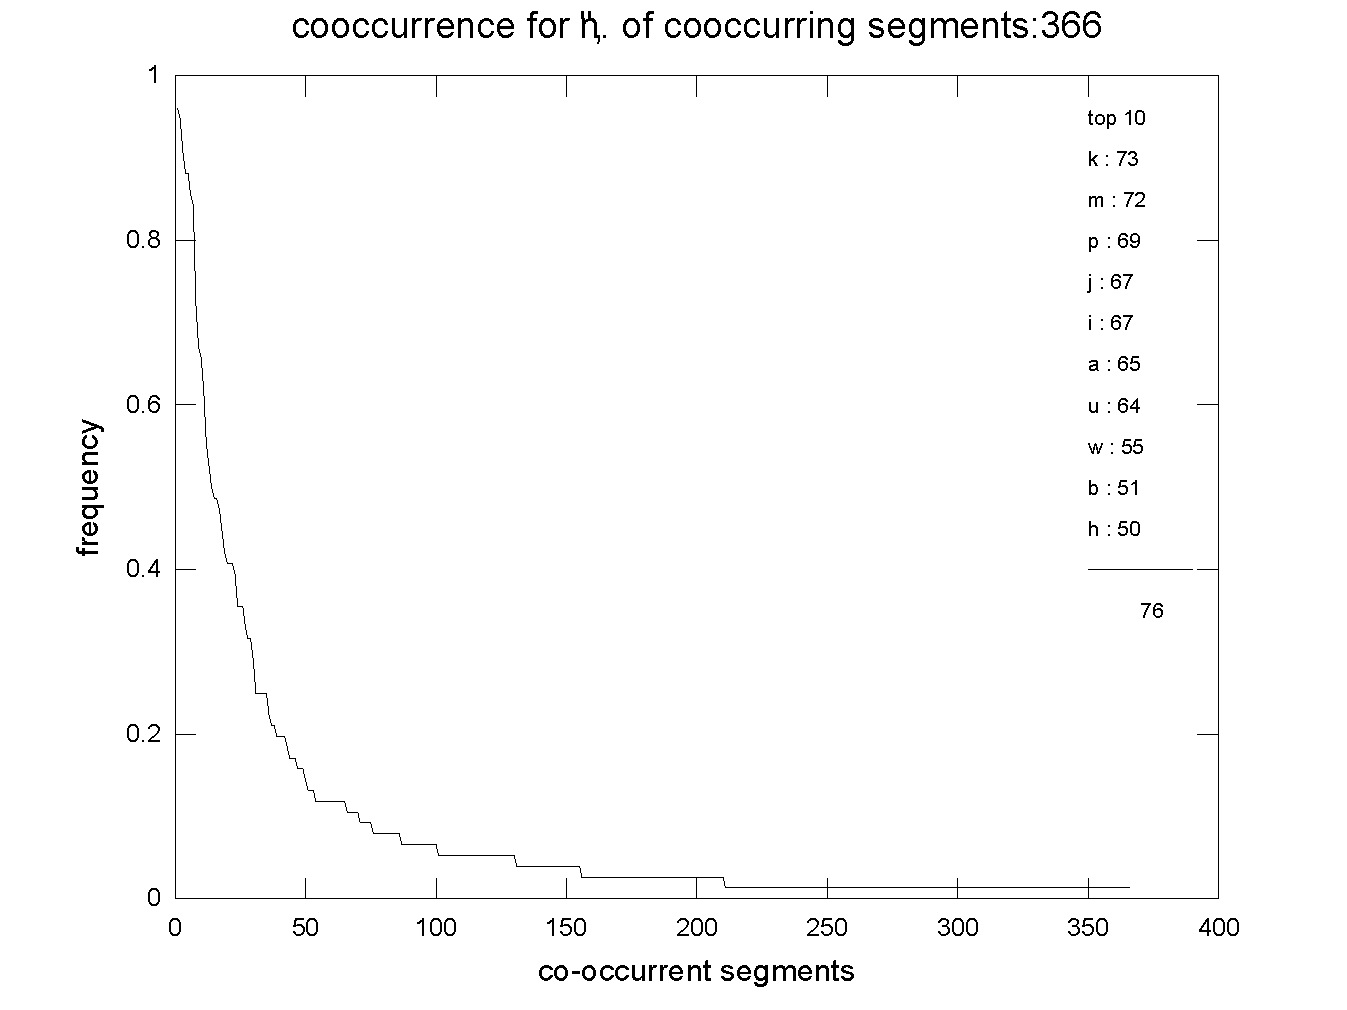
\includegraphics[width=0.45\textwidth]{images/cooccurrence_01.pdf}}                
  \subfloat[This graph presents the co-occurrence frequency for phones in relation to \textipa{[t]}. The phone \textipa{[k]} has a frequency of 96.1\%. \textipa{[m]} follows with 93.3\% and \textipa{[a]} with 91.2\%. 55.6\% of the phones in UPSID are co-occurring with the phone \textipa{[t]}.]{\label{fig:cooccurrence_02}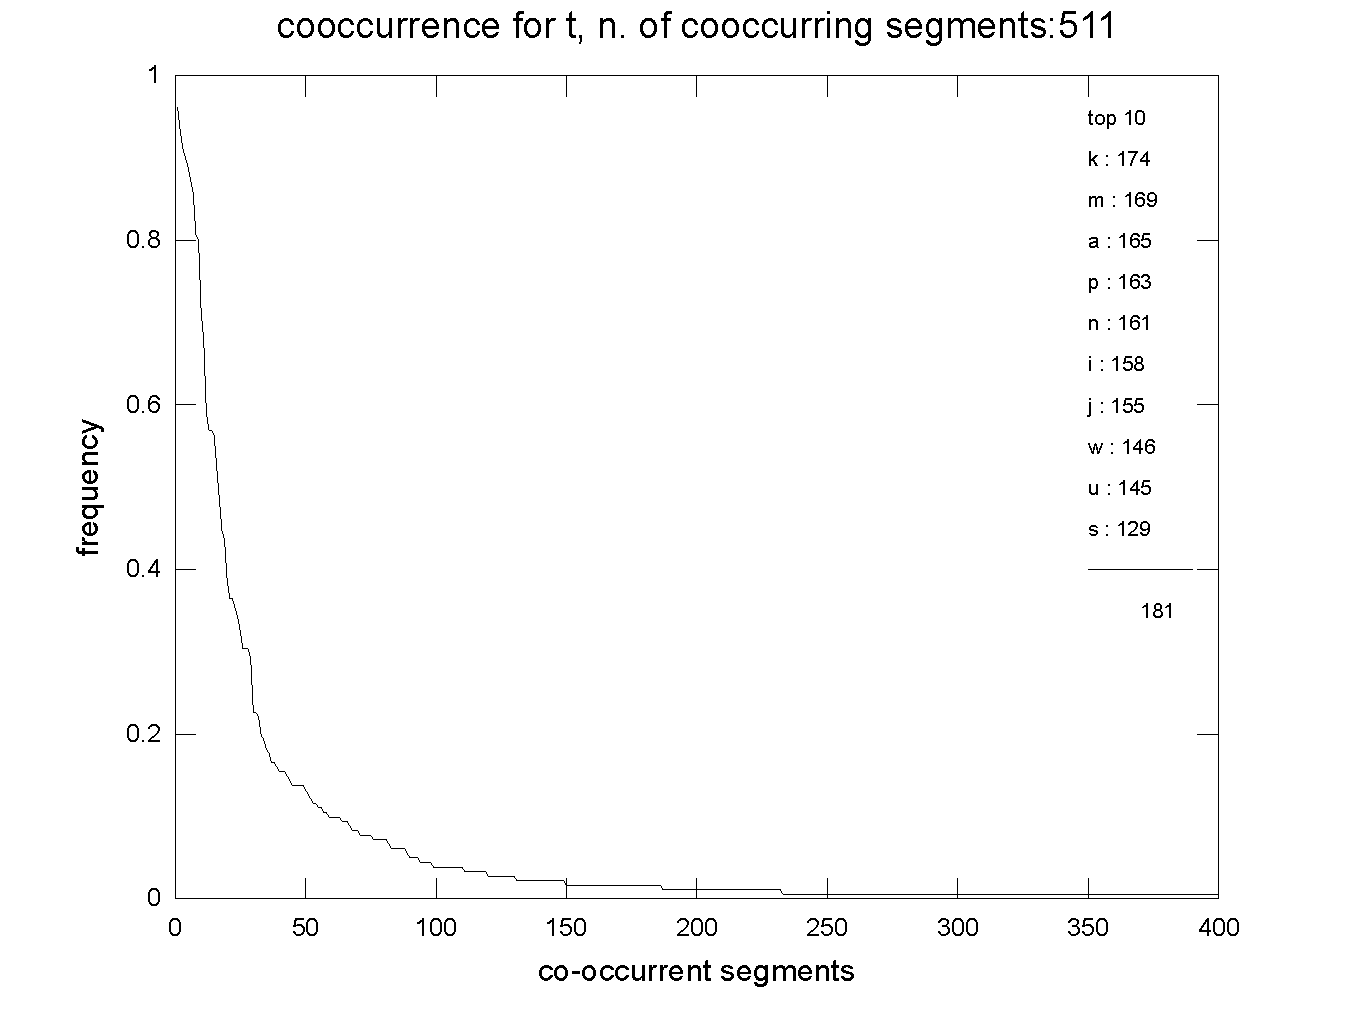
\includegraphics[width=0.45\textwidth]{images/cooccurrence_02.pdf}} \\
  \subfloat[This graph presents the co-occurrence frequency for phones in relation to \textipa{[n]}. The phone \textipa{[m]} has a frequency of 99.0\%. \textipa{[a]} follows with 89.6\% and \textipa{[j]} with 89.1\%. 60.5\% of the phones in UPSID are co-occurring with the phone \textipa{[n]}.]{\label{fig:cooccurrence_03}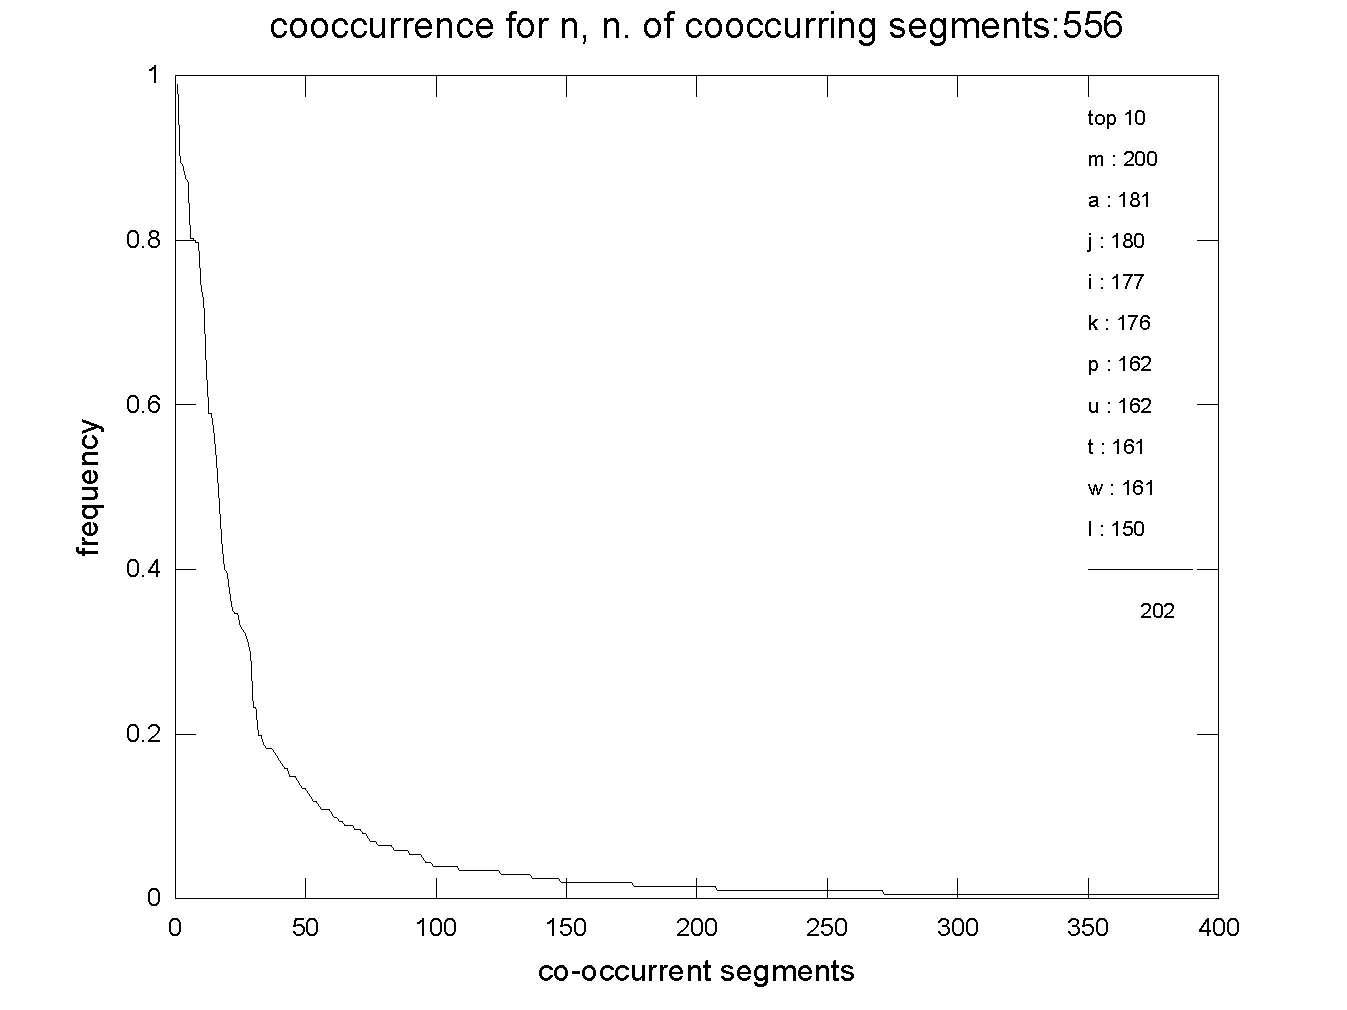
\includegraphics[width=0.45\textwidth]{images/cooccurrence_03.pdf}}
  \subfloat[This graph presents the co-occurrence frequency for phones in relation to \textipa{[l]}. The phone \textipa{[m]} has a frequency of 97.3\%. \textipa{[j]} follows with 91.9\% and \textipa{[k]} with 86.5\%. 38.8\% of the phones in UPSID are co-occurring with the phone \textipa{[l]}.]{\label{fig:cooccurrence_04}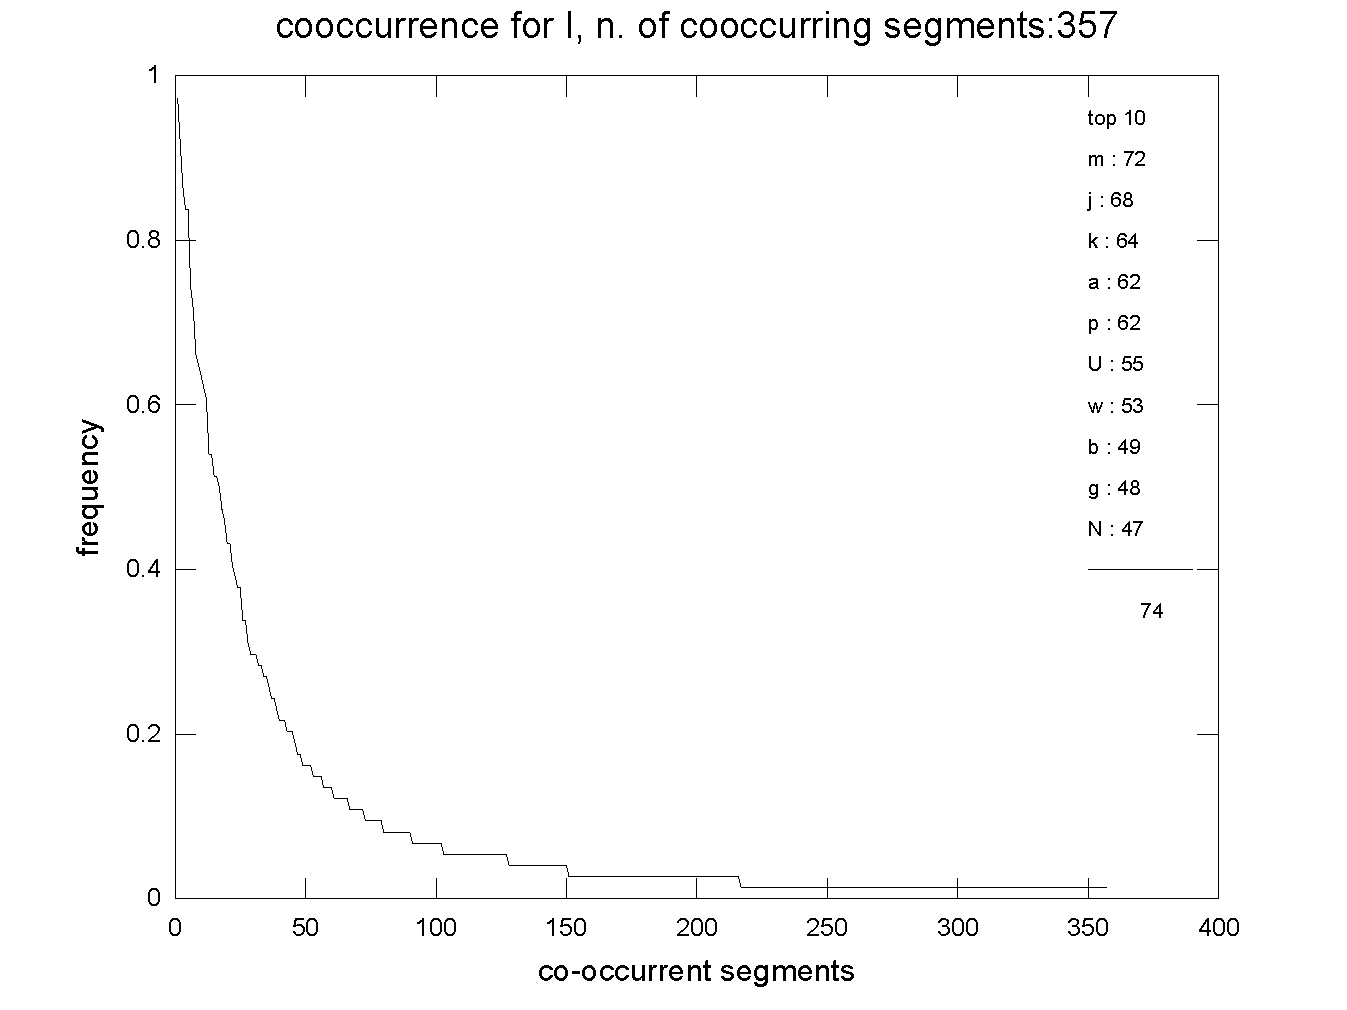
\includegraphics[width=0.45\textwidth]{images/cooccurrence_04.pdf}} \\
  \subfloat[This graph presents the co-occurrence frequency for phones in relation to \textipa{[s]}. The phone \textipa{[m]} has a frequency of 95.4\%. \textipa{[j]} follows with 89.3\% and \textipa{[a]} with 88.3\%. 62.0\% of the phones in UPSID are co-occurring with the phone \textipa{[s]}.]{\label{fig:cooccurrence_05}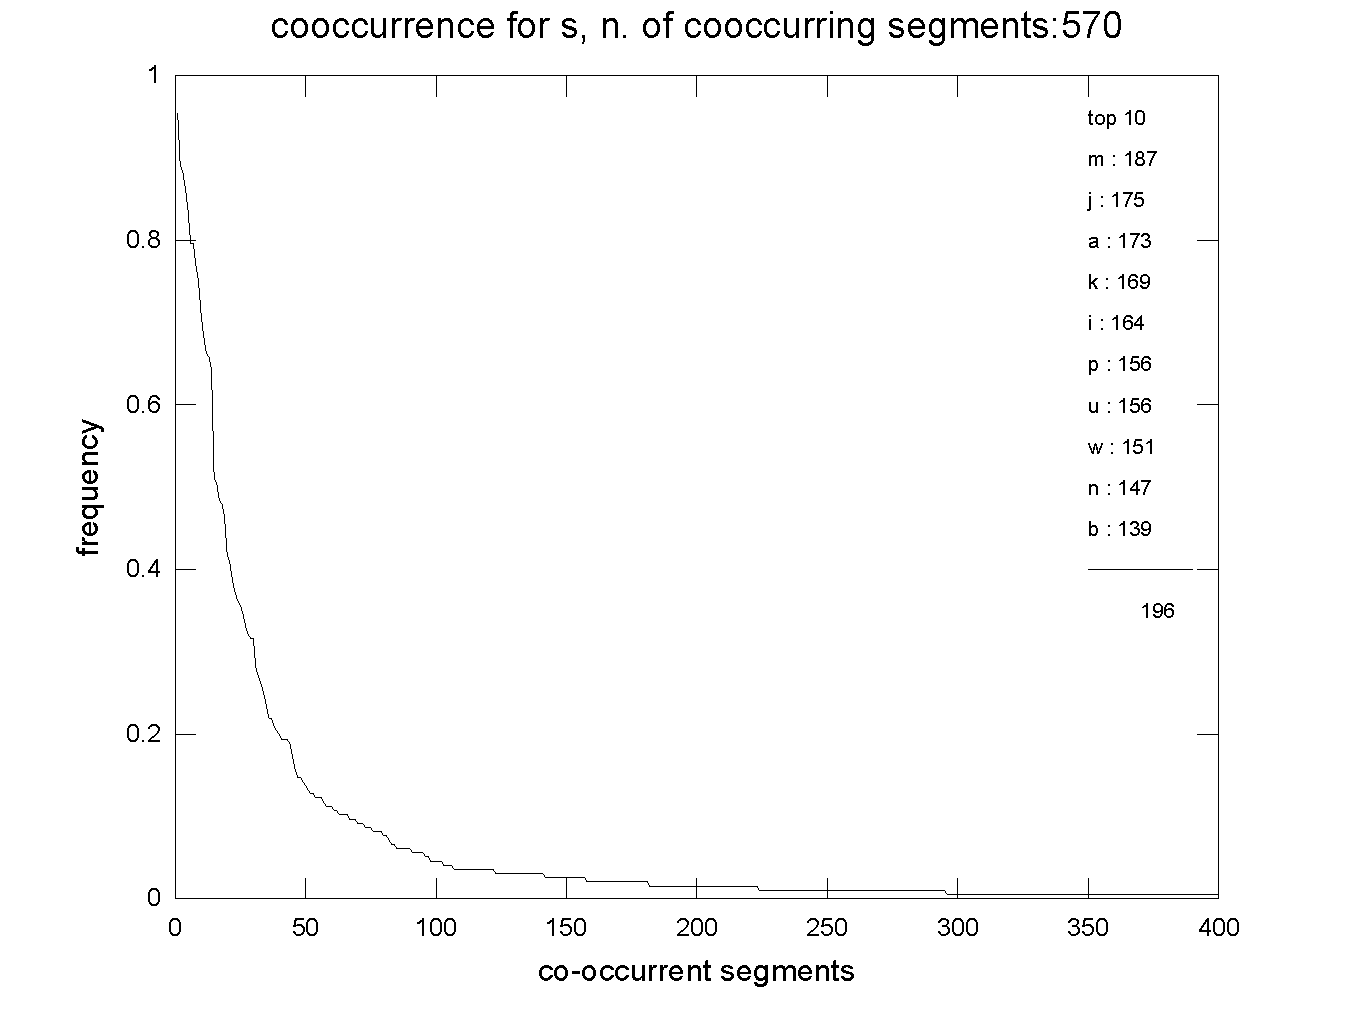
\includegraphics[width=0.45\textwidth]{images/cooccurrence_05.pdf}} 
  \subfloat[This graph presents the co-occurrence frequency for phones in relation to \textipa{[z]}. The phone \textipa{[s]} has a frequency of 100\%. \textipa{[m]} follows with 98.4\% and \textipa{[j]} with 93.5\%. 40.4\% of the phones in UPSID are co-occurring with the phone \textipa{[z]}.]{\label{fig:cooccurrence_06}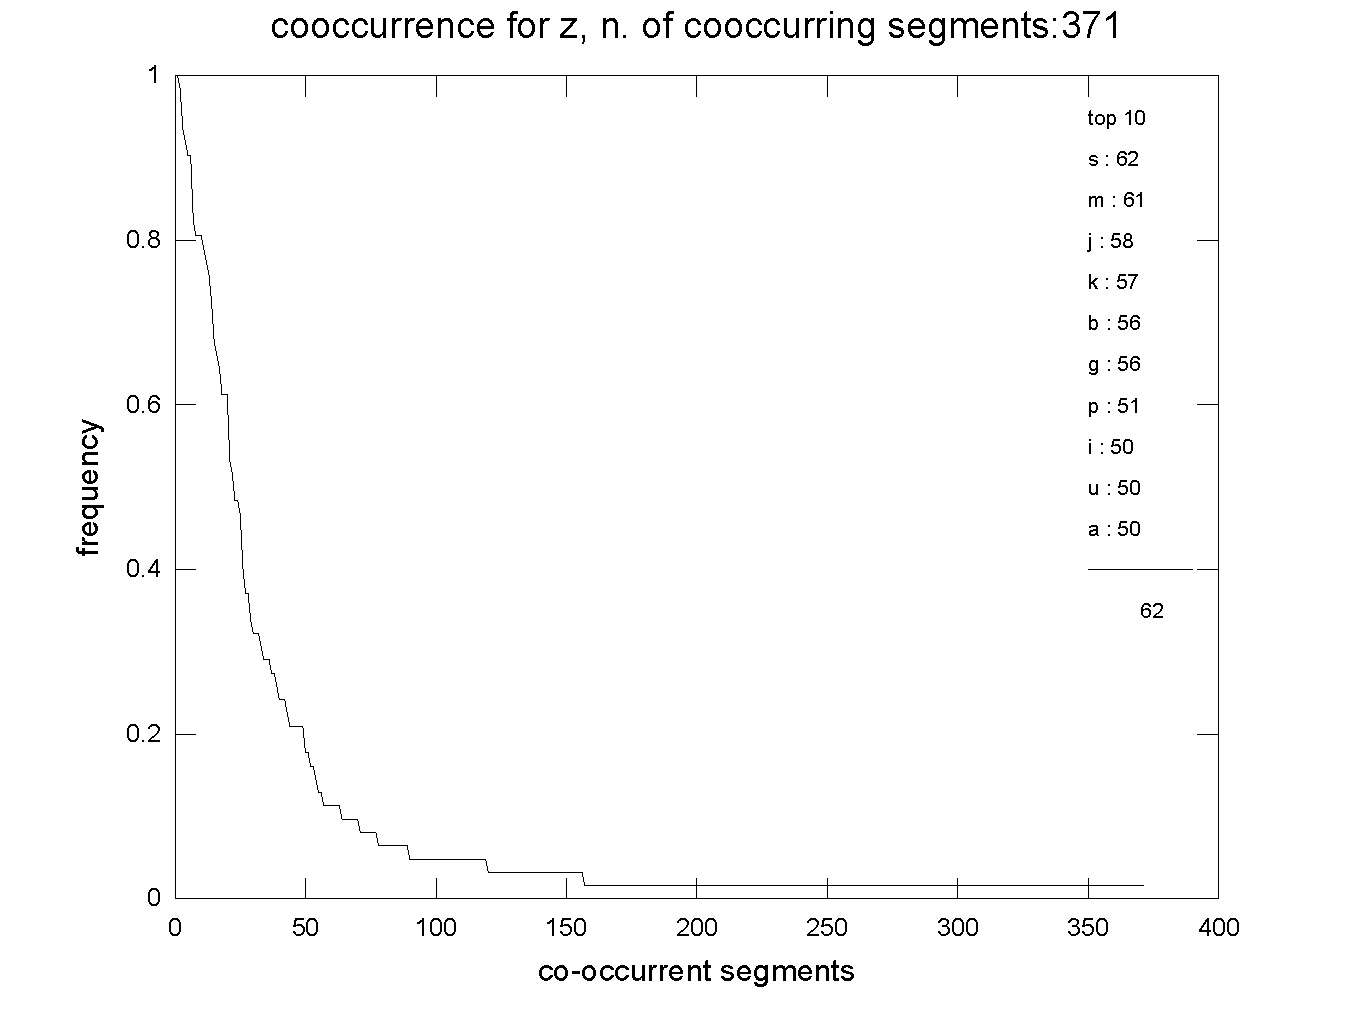
\includegraphics[width=0.45\textwidth]{images/cooccurrence_06.pdf}} 
  \caption{The frequency co-occurrence plots above are derived from the UPSID.}
  \label{fig:cooccurrence}
\end{figure*}


\begin{table}[h]
\caption{List of phones and their top 10 co-occurring pairs with their relative frequency of occurrence (data from UPSID).}
\label{tbl:cooccurrence}
\begin{scriptsize}
\begin{tabular}{|c||c|c|c|c|c|c|c|c|c|c|c|}
\hline 
phone & \multicolumn{10}{|c|}{co-occurring phone with their respective relative frequency (\%)} \\  
\hline 
\textipa{@} & \textipa{k} : 96.1 & \textipa{m} : 94.7 & \textipa{p} : 90.8 & \textipa{j} : 88.2 & \textipa{i} : 88.2 & \textipa{a} : 85.5 & \textipa{u} : 84.2 & \textipa{w} : 72.4 & \textipa{b} : 67.1 & \textipa{h} : 65.8 \\ \hline
\textipa{t} & \textipa{k} : 96.1 & \textipa{m} : 93.4 & \textipa{a} : 91.2 & \textipa{p} : 90.1 & \textipa{n} : 89.0 & \textipa{i} : 87.3 & \textipa{j} : 85.6 & \textipa{w} : 80.7 & \textipa{u} : 80.1 & \textipa{s} : 71.3 \\ \hline
\textipa{n} & \textipa{m} : 99.0 & \textipa{a} : 89.6 & \textipa{j} : 89.1 & \textipa{i} : 87.6 & \textipa{k} : 87.1 & \textipa{p} : 80.2 & \textipa{u} : 80.2 & \textipa{t} : 79.7 & \textipa{w} : 79.7 & \textipa{l} : 74.3 \\ \hline
\textipa{I} & \textipa{m} : 97.3 & \textipa{j} : 91.9 & \textipa{k} : 86.5 & \textipa{a} : 83.8 & \textipa{p} : 83.8 & \textipa{U} : 74.3 & \textipa{w} : 71.6 & \textipa{b} : 66.2 & \textipa{g} : 64.9 & \textipa{N} : 63.5 \\ \hline
\textipa{s} & \textipa{m} : 95.4 & \textipa{j} : 89.3 & \textipa{a} : 88.3 & \textipa{k} : 86.2 & \textipa{i} : 83.7 & \textipa{p} : 79.6 & \textipa{u} : 79.6 & \textipa{w} : 77.0 & \textipa{n} : 75.0 & \textipa{b} : 70.9 \\ \hline
\textipa{z} & \textipa{s} : 100.0 & \textipa{m} : 98.4 & \textipa{j} : 93.5 & \textipa{k} : 91.9 & \textipa{b} : 90.3 & \textipa{g} : 90.3 & \textipa{p} : 82.3 & \textipa{i} : 80.6 & \textipa{u} : 80.6 & \textipa{a} : 80.6 \\ \hline
\textipa{d} & \textipa{b} : 96.7 & \textipa{m} : 94.2 & \textipa{i} : 91.7 & \textipa{a} : 90.8 & \textipa{j} : 90.0 & \textipa{n} : 89.2 & \textipa{g} : 87.5 & \textipa{u} : 86.7 & \textipa{t} : 85.8 & \textipa{k} : 84.2 \\ \hline
\textipa{l} & \textipa{m} : 98.9 & \textipa{j} : 89.1 & \textipa{k} : 86.8 & \textipa{n} : 86.2 & \textipa{a} : 86.2 & \textipa{i} : 85.6 & \textipa{p} : 81.0 & \textipa{w} : 79.9 & \textipa{u} : 79.9 & \textipa{s} : 72.4 \\ \hline
\textipa{i} & \textipa{m} : 93.9 & \textipa{u} : 91.6 & \textipa{k} : 89.6 & \textipa{a} : 89.1 & \textipa{p} : 82.7 & \textipa{j} : 82.7 & \textipa{w} : 73.8 & \textipa{b} : 65.1 & \textipa{h} : 62.6 & \textipa{g} : 57.5 \\ \hline
\textipa{\|[d} & \textipa{b} : 97.5 & \textipa{m} : 96.2 & \textipa{g} : 93.8 & \textipa{j} : 88.8 & \textipa{k} : 85.0 & \textipa{\|[t} : 83.8 & \textipa{i} : 80.0 & \textipa{p} : 76.2 & \textipa{u} : 72.5 & \textipa{a} : 70.0 \\ \hline
\textipa{m} & \textipa{k} : 89.2 & \textipa{i} : 86.8 & \textipa{a} : 86.6 & \textipa{j} : 85.2 & \textipa{p} : 82.6 & \textipa{u} : 81.6 & \textipa{w} : 74.1 & \textipa{b} : 64.2 & \textipa{h} : 61.6 & \textipa{g} : 56.7 \\ \hline
\textipa{n} & \textipa{m} : 99.0 & \textipa{a} : 89.6 & \textipa{j} : 89.1 & \textipa{i} : 87.6 & \textipa{k} : 87.1 & \textipa{p} : 80.2 & \textipa{u} : 80.2 & \textipa{t} : 79.7 & \textipa{w} : 79.7 & \textipa{l} : 74.3 \\ \hline
\textipa{k} & \textipa{m} : 94.0 & \textipa{p} : 91.3 & \textipa{i} : 87.3 & \textipa{a} : 86.6 & \textipa{j} : 83.4 & \textipa{u} : 82.1 & \textipa{w} : 73.2 & \textipa{b} : 62.8 & \textipa{h} : 61.0 & \textipa{g} : 54.1 \\ \hline
\textipa{g} & \textipa{b} : 96.4 & \textipa{m} : 95.3 & \textipa{i} : 89.3 & \textipa{j} : 87.4 & \textipa{k} : 86.2 & \textipa{u} : 84.2 & \textipa{a} : 83.0 & \textipa{p} : 76.7 & \textipa{w} : 72.3 & \textipa{h} : 63.6 \\ \hline
\textipa{p} & \textipa{k} : 98.1 & \textipa{m} : 93.6 & \textipa{a} : 87.2 & \textipa{i} : 86.7 & \textipa{j} : 82.9 & \textipa{u} : 81.3 & \textipa{w} : 71.7 & \textipa{b} : 60.5 & \textipa{h} : 60.3 & \textipa{N} : 54.4 \\ \hline
\textipa{b} & \textipa{m} : 95.1 & \textipa{i} : 89.2 & \textipa{k} : 88.2 & \textipa{j} : 86.8 & \textipa{g} : 85.0 & \textipa{u} : 84.3 & \textipa{a} : 84.3 & \textipa{p} : 79.1 & \textipa{w} : 72.5 & \textipa{h} : 65.9 \\ \hline
\textipa{S} & \textipa{m} : 94.7 & \textipa{j} : 91.4 & \textipa{k} : 88.8 & \textipa{i} : 84.0 & \textipa{a} : 82.9 & \textipa{p} : 80.2 & \textipa{u} : 78.1 & \textipa{w} : 74.3 & \textipa{h} : 73.3 & \textipa{b} : 68.4 \\ \hline
\textipa{Z} & \textipa{S} : 95.1 & \textipa{m} : 95.1 & \textipa{j} : 90.2 & \textipa{k} : 90.2 & \textipa{b} : 82.0 & \textipa{g} : 80.3 & \textipa{i} : 78.7 & \textipa{p} : 78.7 & \textipa{u} : 77.0 & \textipa{a} : 70.5 \\ \hline
\end{tabular} 
\end{scriptsize}
\end{table}


%@ : k 96.1   m 94.7   p 90.8   j 88.2   i 88.2   a 85.5   u 84.2   w 72.4   b 67.1   h 65.8
%t : k 96.1   m 93.4   a 91.2   p 90.1   n 89.0   i 87.3   j 85.6   w 80.7   u 80.1   s 71.3   
%n : m 99.0   a 89.6   j 89.1   i 87.6   k 87.1   p 80.2   u 80.2   t 79.7   w 79.7   l 74.3   
%I : m 97.3   j 91.9   k 86.5   a 83.8   p 83.8   U 74.3   w 71.6   b 66.2   g 64.9   N 63.5   
%s : m 95.4   j 89.3   a 88.3   k 86.2   i 83.7   p 79.6   u 79.6   w 77.0   n 75.0   b 70.9   
%z : s 100.0   m 98.4   j 93.5   k 91.9   b 90.3   g 90.3   p 82.3   i 80.6   u 80.6   a 80.6   
%d : b 96.7   m 94.2   i 91.7   a 90.8   j 90.0   n 89.2   g 87.5   u 86.7   t 85.8   k 84.2   
%l : m 98.9   j 89.1   k 86.8   n 86.2   a 86.2   i 85.6   p 81.0   w 79.9   u 79.9   s 72.4   
%i : m 93.9   u 91.6   k 89.6   a 89.1   p 82.7   j 82.7   w 73.8   b 65.1   h 62.6   g 57.5   
%dD : b 97.5   m 96.2   g 93.8   j 88.8   k 85.0   tD 83.8   i 80.0   p 76.2   u 72.5   a 70.0   
%m : k 89.2   i 86.8   a 86.6   j 85.2   p 82.6   u 81.6   w 74.1   b 64.2   h 61.6   g 56.7   
%n : m 99.0   a 89.6   j 89.1   i 87.6   k 87.1   p 80.2   u 80.2   t 79.7   w 79.7   l 74.3   
%k : m 94.0   p 91.3   i 87.3   a 86.6   j 83.4   u 82.1   w 73.2   b 62.8   h 61.0   g 54.1   
%g : b 96.4   m 95.3   i 89.3   j 87.4   k 86.2   u 84.2   a 83.0   p 76.7   w 72.3   h 63.6   
%p : k 98.1   m 93.6   a 87.2   i 86.7   j 82.9   u 81.3   w 71.7   b 60.5   h 60.3   N 54.4   
%b : m 95.1   i 89.2   k 88.2   j 86.8   g 85.0   u 84.3   a 84.3   p 79.1   w 72.5   h 65.9   
%S : m 94.7   j 91.4   k 88.8   i 84.0   a 82.9   p 80.2   u 78.1   w 74.3   h 73.3   b 68.4   
%Z : S 95.1   m 95.1   j 90.2   k 90.2   b 82.0   g 80.3   i 78.7   p 78.7   u 77.0   a 70.5 



If we believe that speech symbols repertoires are not chosen randomly, 
we might wonder what guides the choices of a repertoire. 
Not only the way those symbols are arranged, but also the way they are used (combined) 
is important in the process of understanding choices. 
Using the Gutenberg's database transcribed with the CMU pronouncing dictionary, as described above, we might get information 
on phone clusters frequency of occurrence (see also Figure \ref{fig:diphonesfrequency_en}):

\begin{tiny}
\begin{multicols}{4}
\begin{enumerate}
    \item \textipa{@n} : 1296408
    \item \textipa{D@} : 785354
    \item \textipa{nd} : 784028
    \item \textipa{st} : 651129
    \item \textipa{@v} : 489267
    \item \textipa{Or} : 472069
    \item \textipa{In} : 470069
    \item \textipa{tu} : 425544
    \item \textipa{t@} : 420825
    \item \textipa{IN} : 387096
    \item \textipa{Iz} : 380357
    \item \textipa{@l} : 372847
    \item \textipa{En} : 349905
    \item \textipa{nt} : 337193
    \item \textipa{\ae t} : 284460
    \item \textipa{wI} : 282526
    \item \textipa{@t} : 265396
    \item \textipa{Er} : 264293
    \item \textipa{r@} : 261447
    \item \textipa{It} : 260544
    \item \textipa{@s} : 246996
    \item \textipa{ju} : 245715
    \item \textipa{h\ae} : 237724
    \item \textipa{hI} : 237490
    \item \textipa{@m} : 233793
    \item \textipa{ri} : 219997
    \item \textipa{li} : 219652
    \item \textipa{An} : 213755
    \item \textipa{\ae n} : 213169
    \item \textipa{s@} : 210385
    \item \textipa{Is} : 208619
    \item \textipa{D\ae} : 194602
    \item \textipa{@f} : 193570
    \item \textipa{Ar} : 193525
	\item[] $\vdots$
	\item[1120] \textipa{uaI} : 1
	\item[1121] \textipa{OIA} : 1
	\item[1122] \textipa{bS} : 1
	\item[1123] \textipa{pv} : 1
	\item[1124] \textipa{iU} : 1
	\item[1125] \textipa{EoU} : 1
\end{enumerate}
\end{multicols}
\end{tiny}



\begin{figure}[h!]
\centering
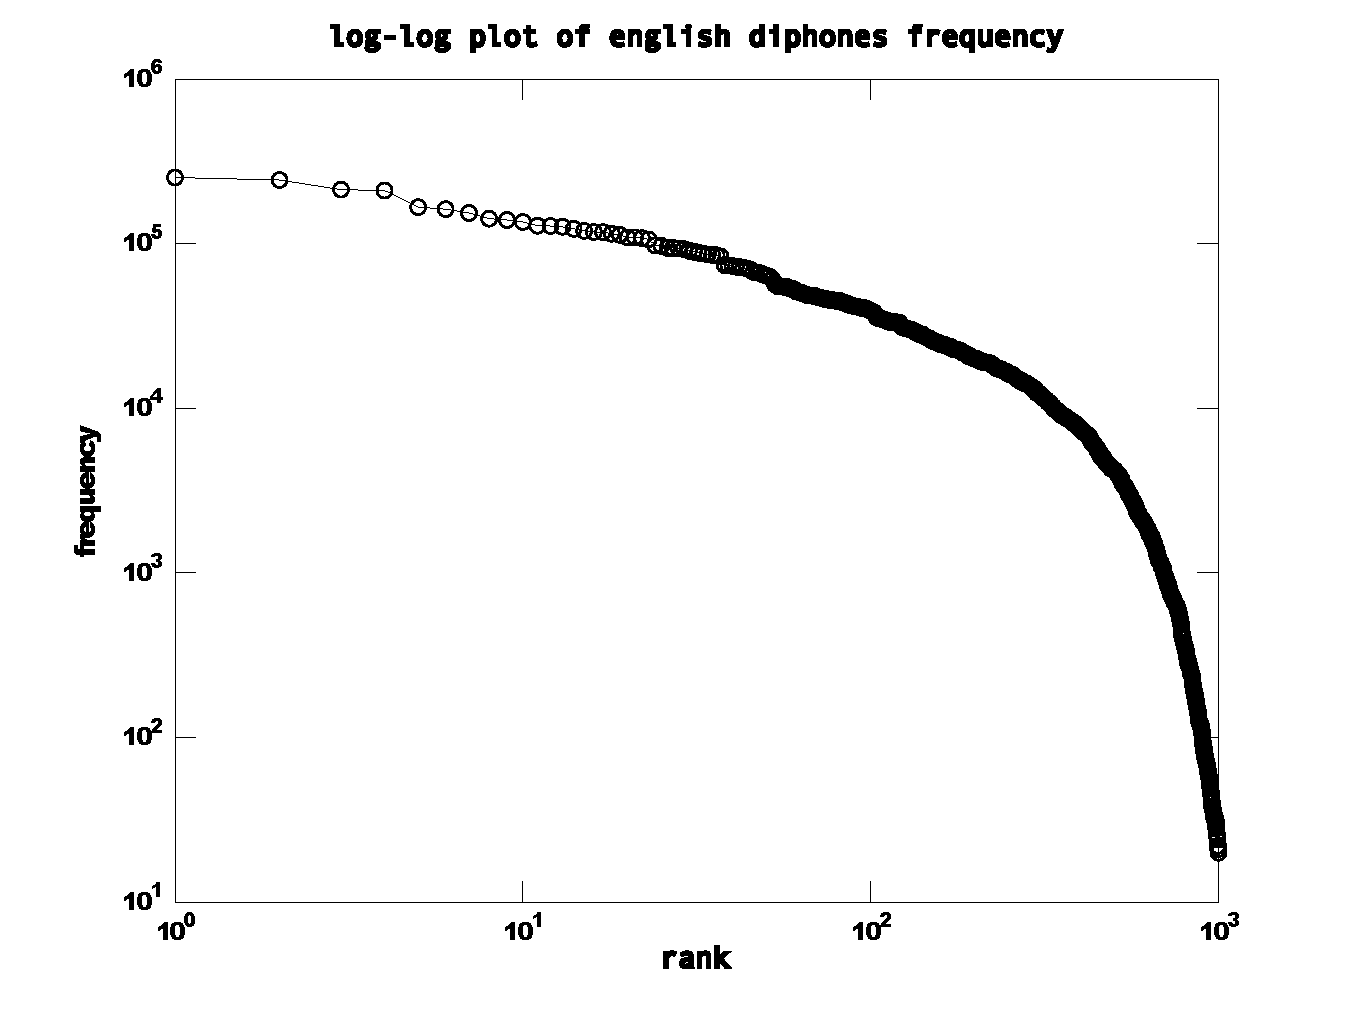
\includegraphics[width=0.75\textwidth]{images/diphonesfrequency_en.pdf}
\caption{Log-log plot of the diphones frequency of occurrence versus their rank.}
\label{fig:diphonesfrequency_en}
\end{figure} 




Normalizing the frequency of occurrence of each diphone by the frequency of occurrence of each phone that is part of them, we get a different ordering that is displayed in the list bellow, and illustrated by the log-log plot in Figure \ref{fig:diphonesnormalizedfrequencyresorted_en}.

\begin{tiny}
\begin{multicols}{6}
\begin{enumerate}
    \item \textipa{Z@}
    \item \textipa{D@}
    \item \textipa{@v}
    \item \textipa{S@} 
    \item \textipa{dZ@}
    \item \textipa{b@}
    \item \textipa{@l}
    \item \textipa{@f}
    \item \textipa{ju} 
    \item \textipa{@m}
    \item \textipa{Or}
    \item \textipa{@b}
    \item \textipa{@tS}
    \item \textipa{nd}
    \item \textipa{k@} 
    \item \textipa{@g}
    \item \textipa{@p}
    \item $\vdots$
	\item[1120] \textipa{zs}
	\item[1121] \textipa{uaI}
	\item[1122] \textipa{aIh}
	\item[1123] \textipa{EoU}
	\item[1124] \textipa{ddZ}
	\item[1125] \textipa{tv}
\end{enumerate}
\end{multicols}
\end{tiny}


\begin{figure}[h!]
\centering
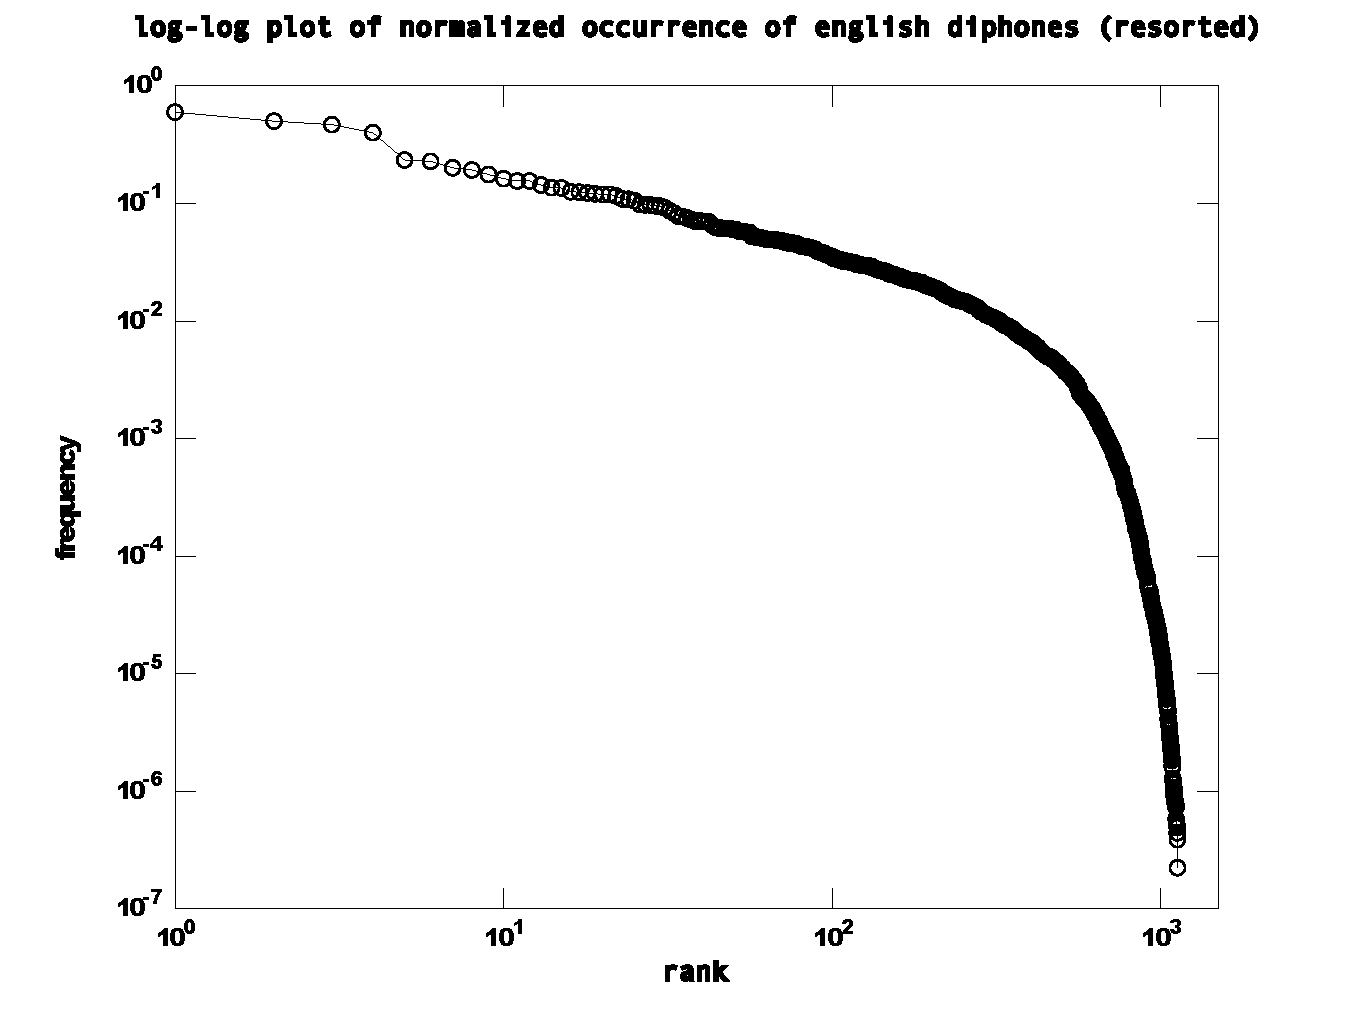
\includegraphics[width=0.75\textwidth]{images/diphonesnormalizedfrequencyresorted_en.pdf}
\caption{Log-log plot of the diphones normalized frequency of occurrence versus their rank. The normalization is made using the frequency of occurrence of each phone in the pair.}
\label{fig:diphonesnormalizedfrequencyresorted_en}
\end{figure} 


Using the information on the occurrence of diphones, it is possible to estimate the probability of occurrence of a subsequent phone for each previous occurring phone. Those probabilities were computed and are displayed in Figure \ref{fig:diphones_cond_probability_en} as a matrix. Each entry $(i,j)$ in the matrix refers to the probability of occurrence of phone $j$ followed by phone $i$. The phones in the first position of a diphone (prior phones) are arranged along the y axis of the figure, and the phones in the second position (posterior phone) of the diphone are displayed along the x axis. The phones are arranged according to the their frequency of occurrence in the language. We observe in the figure that the most frequent phones (in the left part of the figure) also have an average higher conditional probability of occurrence regardless which the prior phone is.


\begin{figure}[h!]
\centering
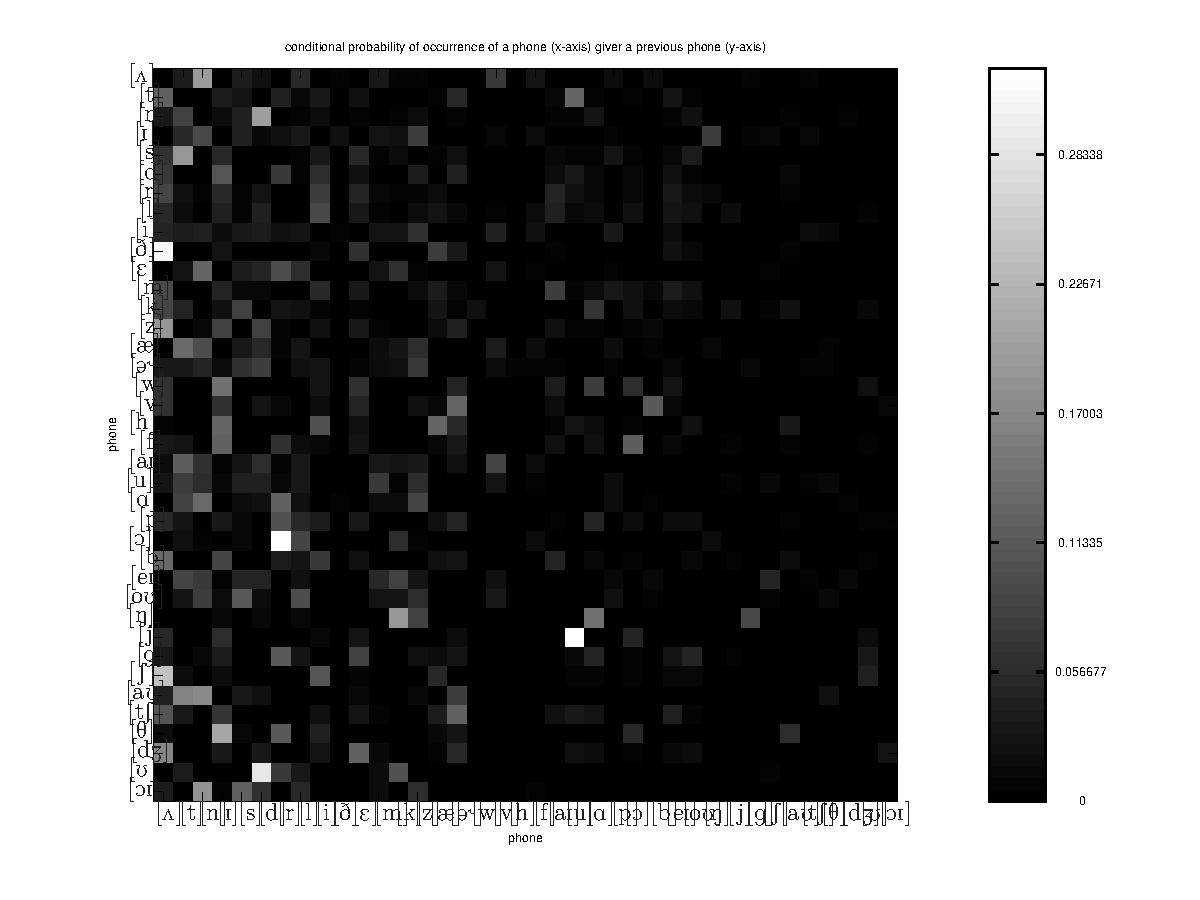
\includegraphics[width=0.75\textwidth]{images/diphones_cond_probability_en.pdf}
\caption{Probability of occurrence of a phone given another previous phone.}
\label{fig:diphones_cond_probability_en}
\end{figure} 



Another analysis here presented consists of computing the number of elements (letters and phones) 
used to build up words. Figure \ref{fig:wordslength_en} shows the number of occurrence of words 
with a certain letter-length. We observe that the peak occurs in 3 letter words. 
Figure \ref{fig:wordsphoneslength_en} is a similar graphic, displaying the number of occurrence 
of words with a certain phone-length. The peak appears in two phone words. For every $L$ symbol 
word made up of a combination of symbols taken from a set of $N$ elements, there are $N^L$ possible 
combinations. 
%Using this number of possible combinations as a normalizing factor, we get the curves 
%displayed in figures \ref{fig:wordslengthfreqnorm_en} and \ref{fig:wordsphoneslengthfreqnorm_en}. 
%If the choices of symbols to build a word were at random, we would expect Figures \ref{fig:wordslength_en} 
%and \ref{fig:wordsphoneslength_en} to be straight lines, what they are clearly not. 
The last two graphics \ref{fig:averagewordslength_en} and \ref{fig:averagewordsphoneslength_en} 
show the average word length across word rank, showing that the most frequent words, on average, 
have a short length; the unusual words are, on average, significantly longer.



\begin{figure*}[p]
  \centering 
  \captionsetup[subfigure]{margin=10pt,singlelinecheck=false}
  \subfloat[Frequency of occurrence of words of a given length (letters).]{\label{fig:wordslength_en}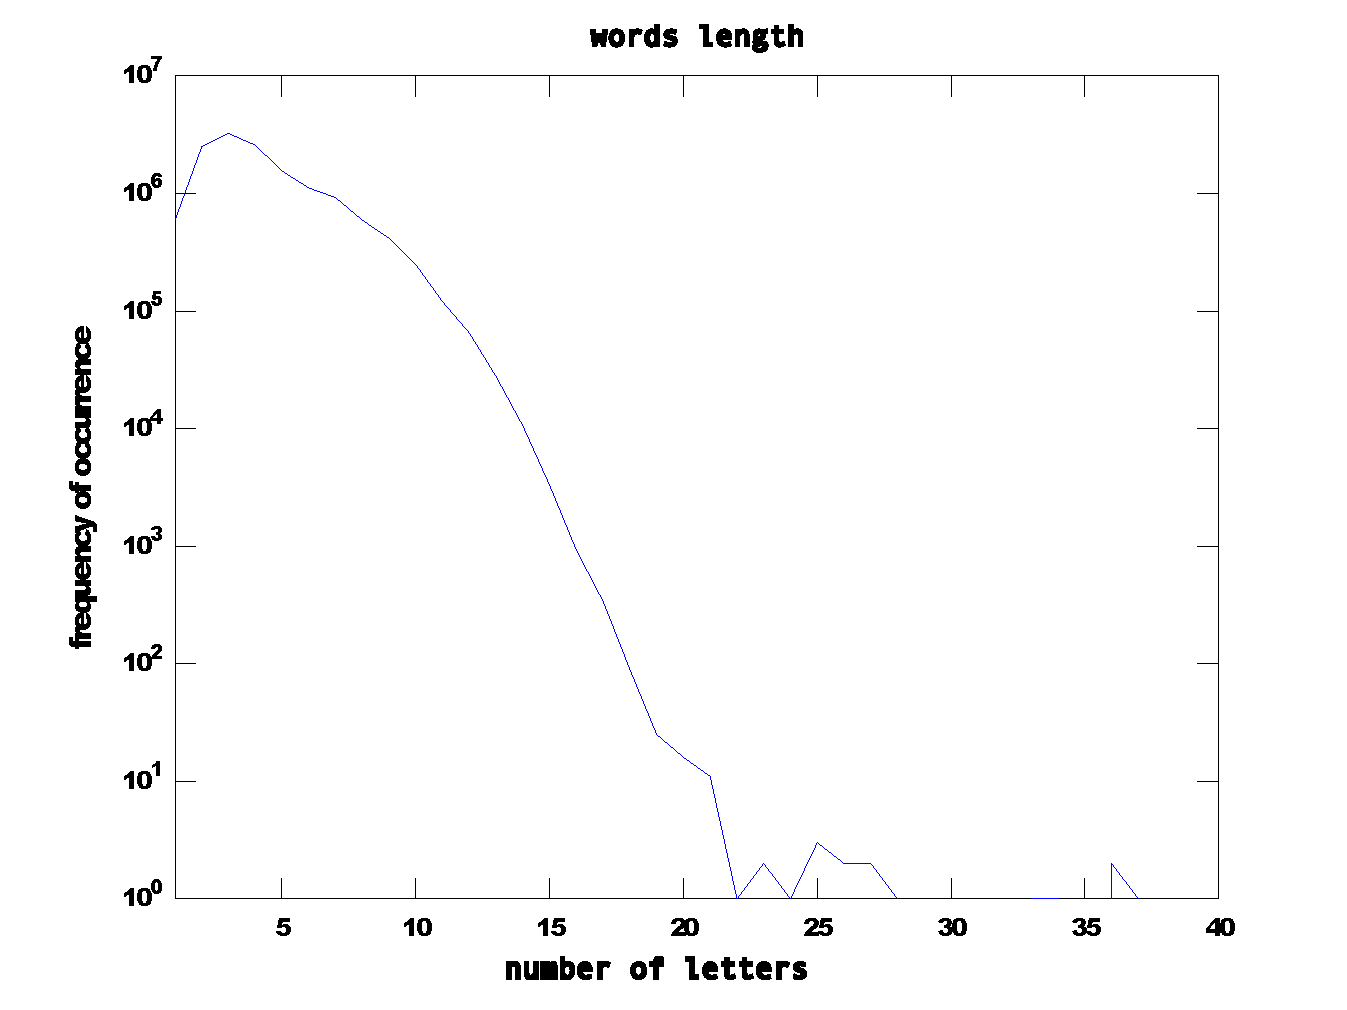
\includegraphics[width=0.45\textwidth]{images/wordslength_en.pdf}}                
  \subfloat[Frequency of occurrence of words of a given length (phones).]{\label{fig:wordsphoneslength_en}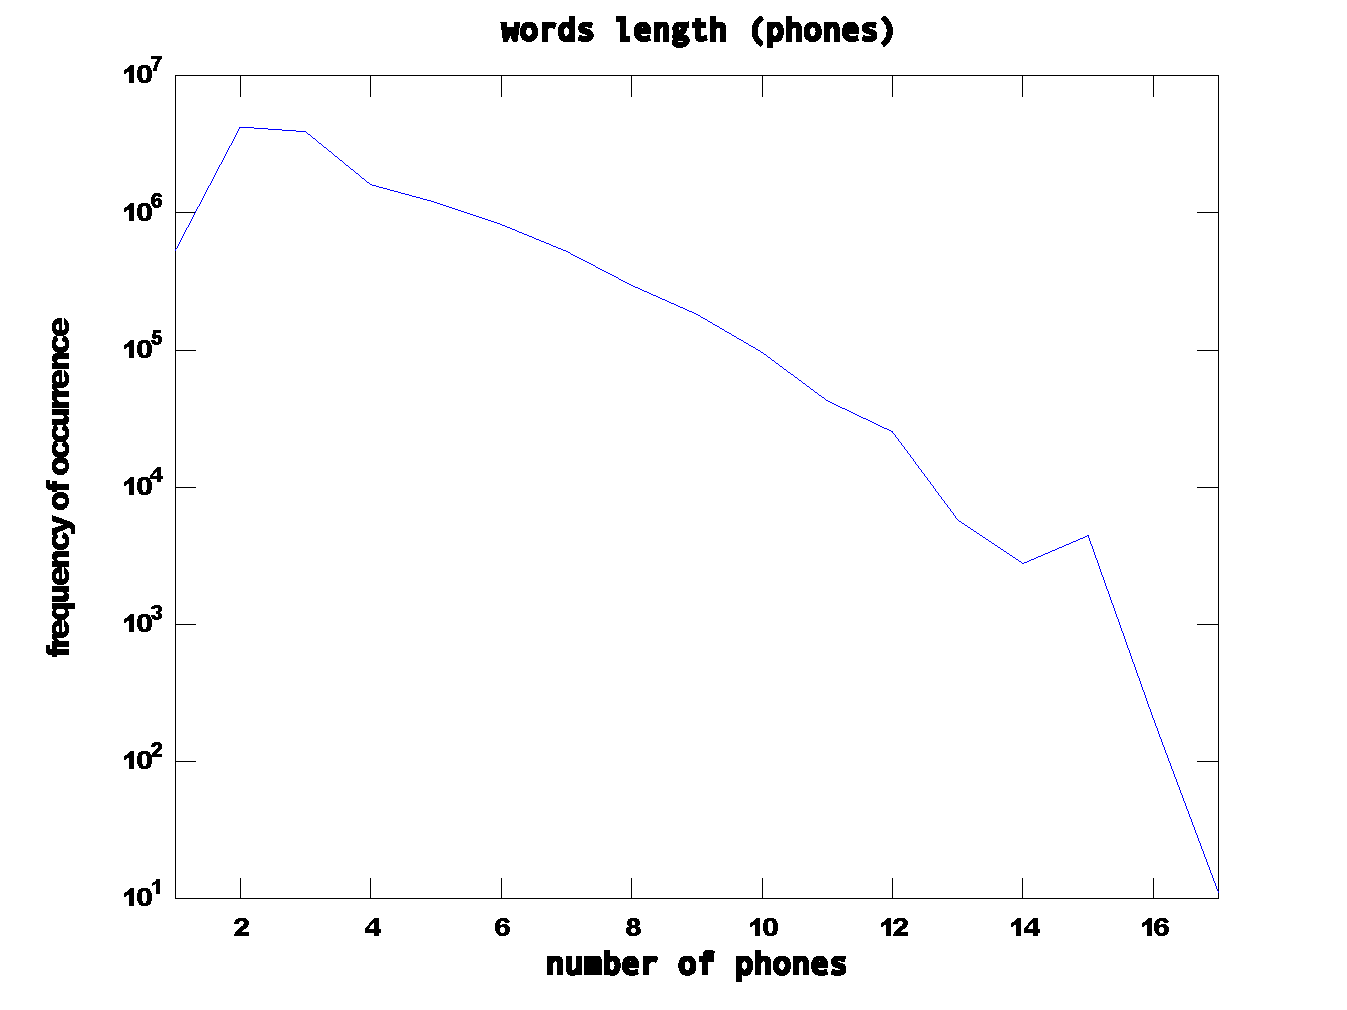
\includegraphics[width=0.45\textwidth]{images/wordsphoneslength_en.pdf}} \\
  %\subfloat[Frequency of occurrence of words of a given length (letters) normalized by the total number of  combinations of letters for a given length.]{\label{fig:wordslengthfreqnorm_en}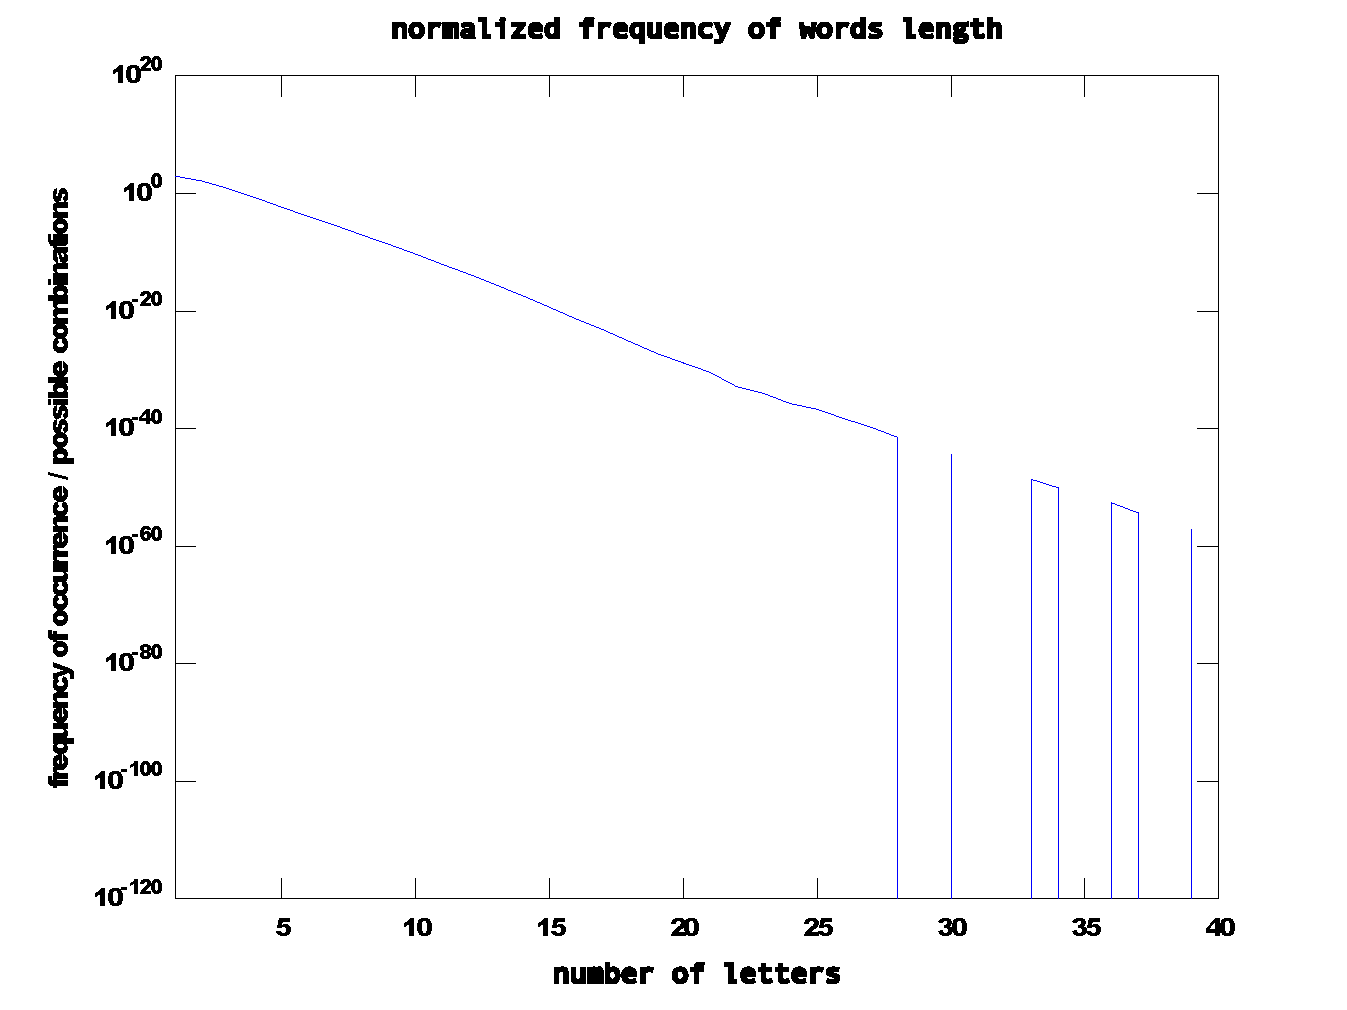
\includegraphics[width=0.45\textwidth]{images/wordslengthfreqnorm_en.pdf}}
  %\subfloat[Frequency of occurrence of words of a given length (phones) normalized by the total number of  combinations of phones for a given length.]{\label{fig:wordsphoneslengthfreqnorm_en}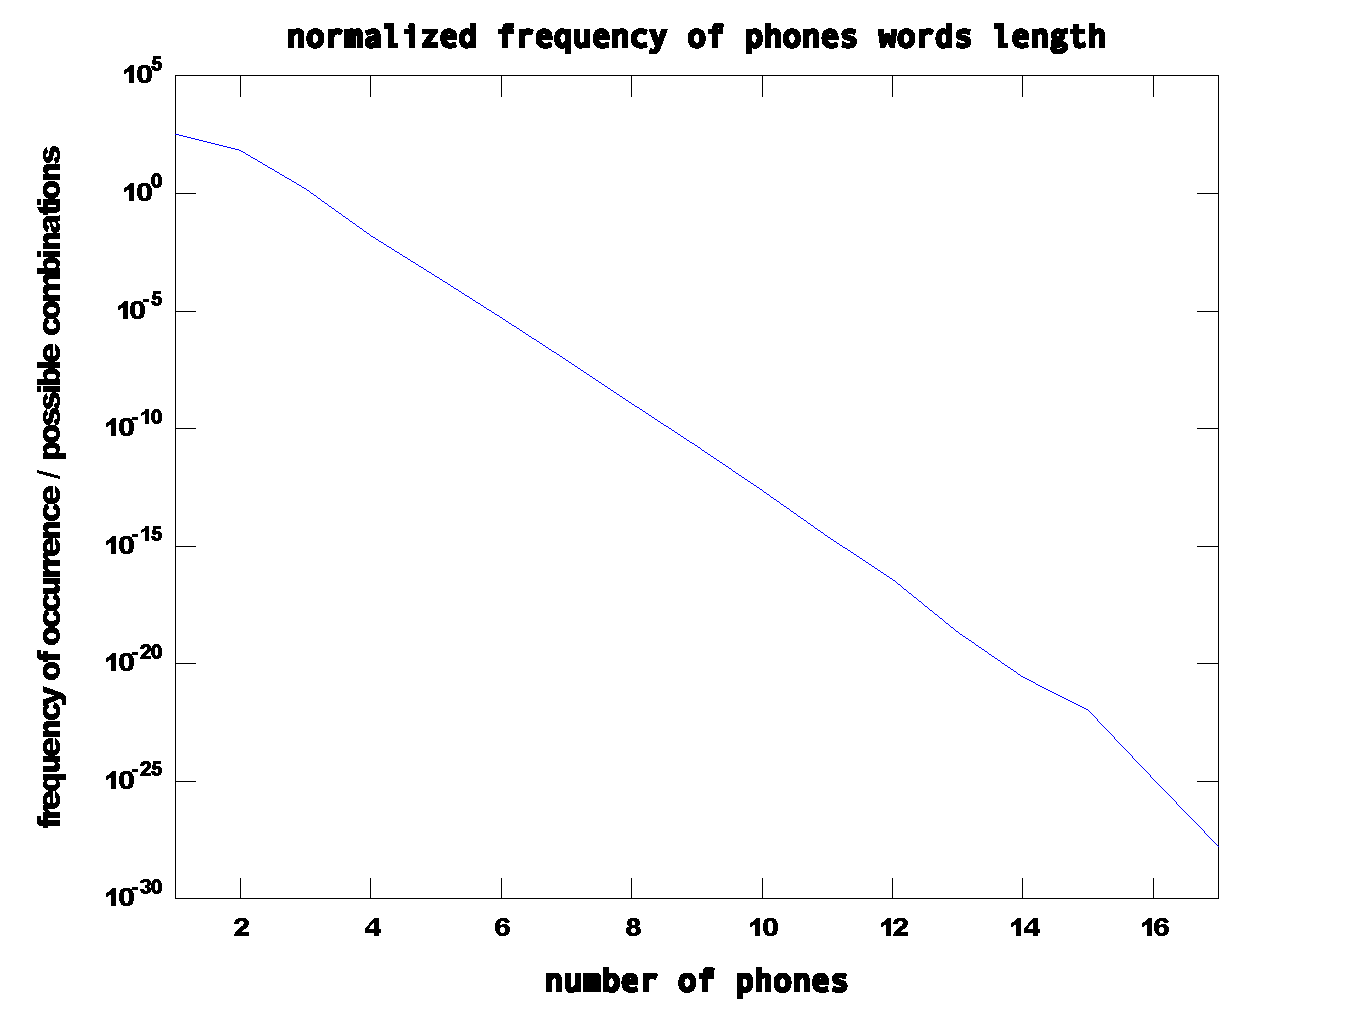
\includegraphics[width=0.45\textwidth]{images/wordsphoneslengthfreqnorm_en.pdf}} \\
  \subfloat[Average word length (letters) across word rank.]{\label{fig:averagewordslength_en}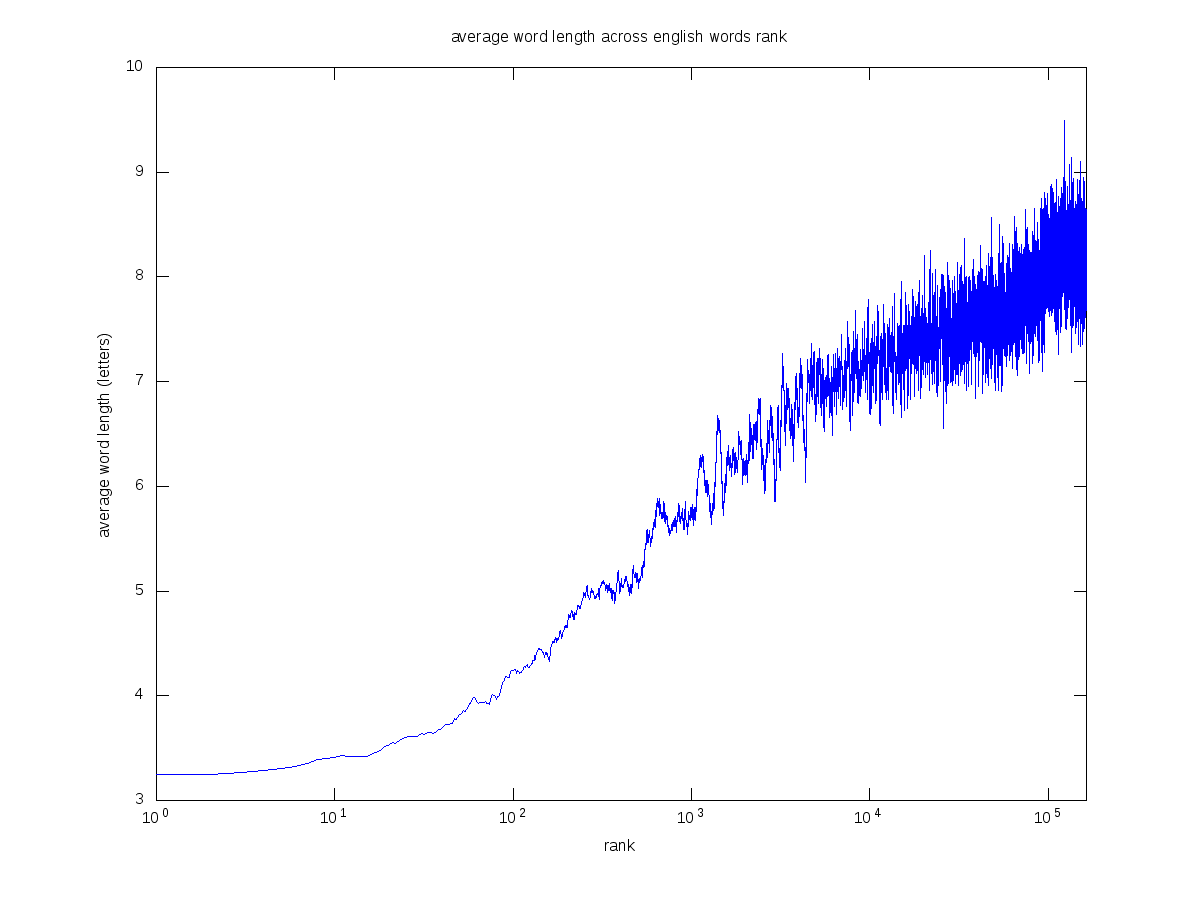
\includegraphics[width=0.45\textwidth]{images/averagewordslength_en.png}} 
  \subfloat[Average word length (phones) across word rank.]{\label{fig:averagewordsphoneslength_en}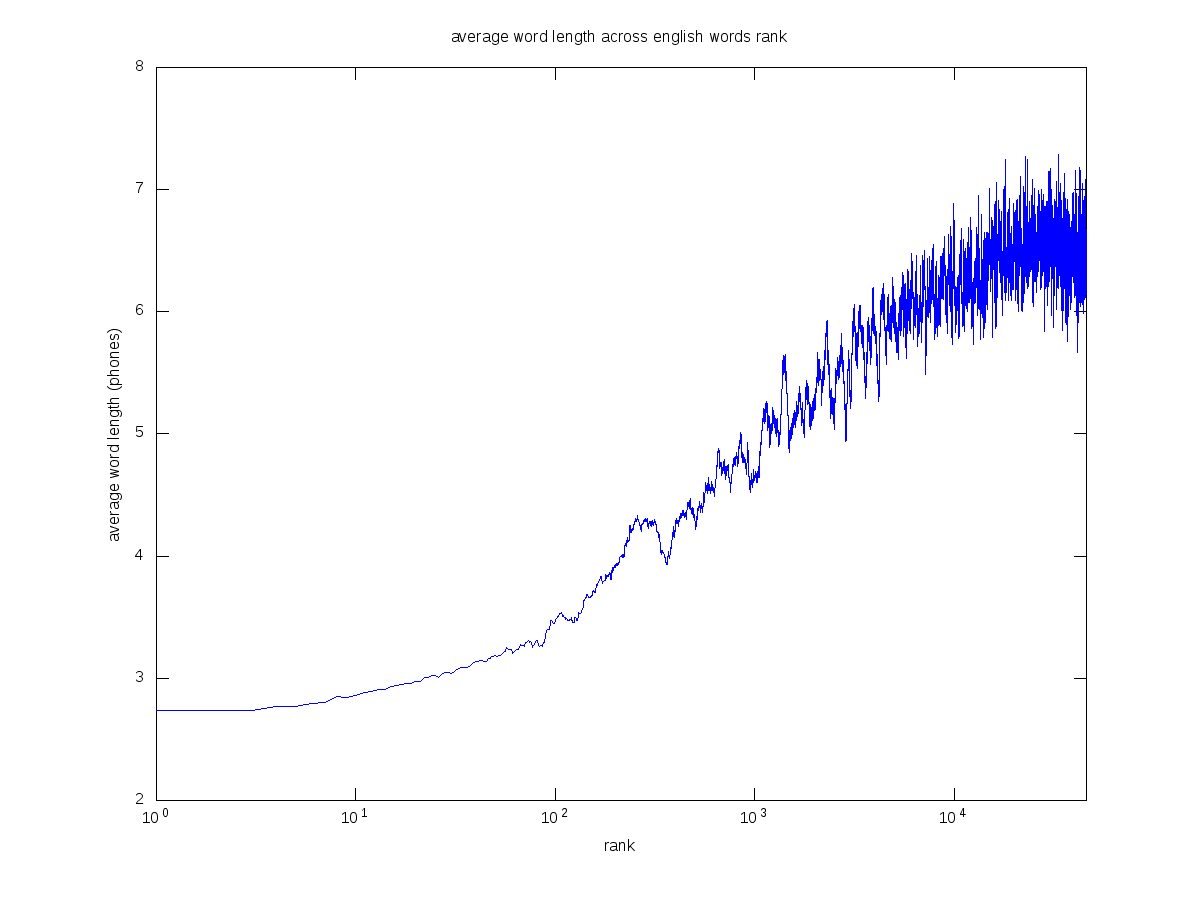
\includegraphics[width=0.45\textwidth]{images/averagewordsphoneslength_en.png}} 
  \caption{Words length statistics (letters and phones) and how it does deviate from a simply random combination of symbols.}
  \label{fig:wordslength}
\end{figure*}




\begin{figure*}[p]
  \centering 
  \captionsetup[subfigure]{margin=10pt,singlelinecheck=false}
  \subfloat[Log-log plot of the frequency of occurrence of words with phone \textipa{[t]} versus their rank.]{\label{fig:zipfwordsphone_T}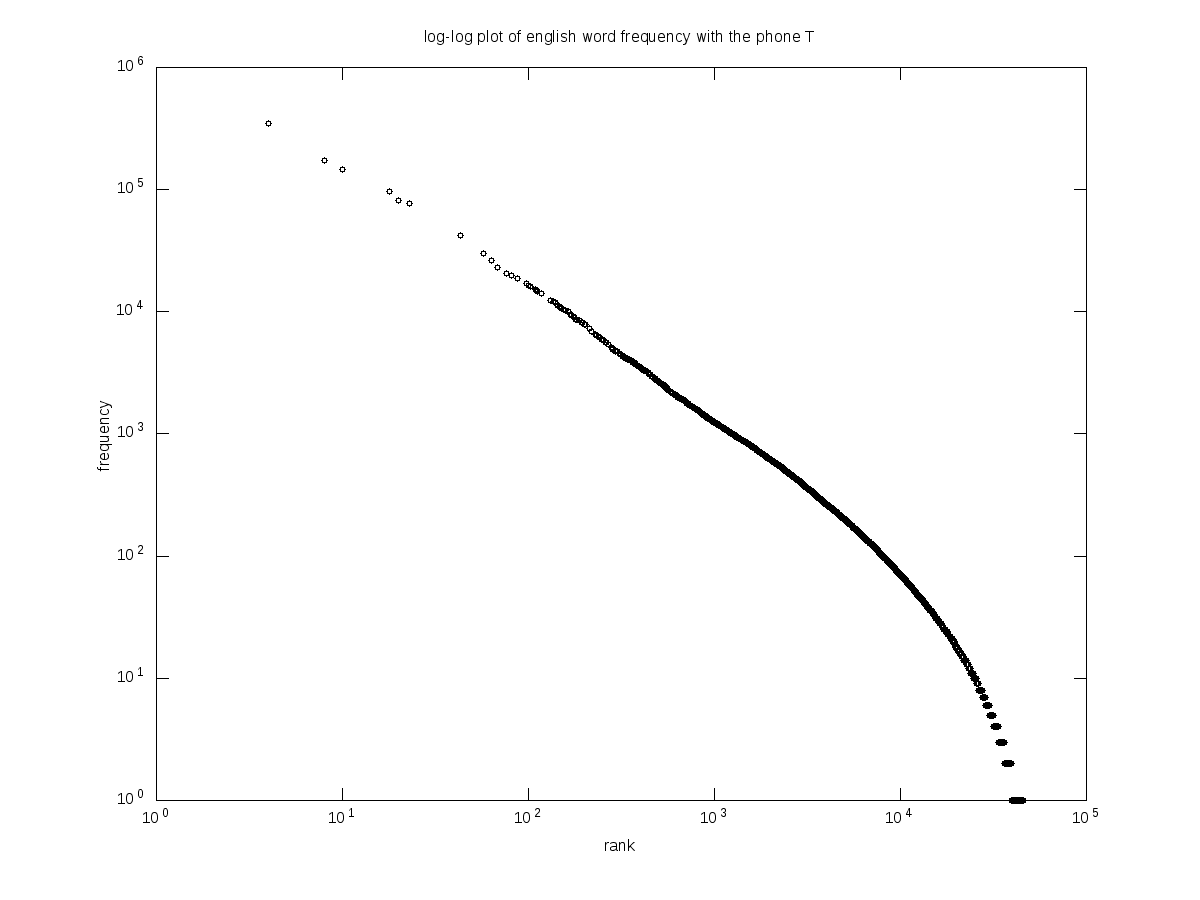
\includegraphics[width=0.45\textwidth]{images/zipfwordsphone_T.png}}                
  \subfloat[Probability of occurrence of words with phone \textipa{[t]} versus the rank of words.]{\label{fig:proboccwordsphone_T}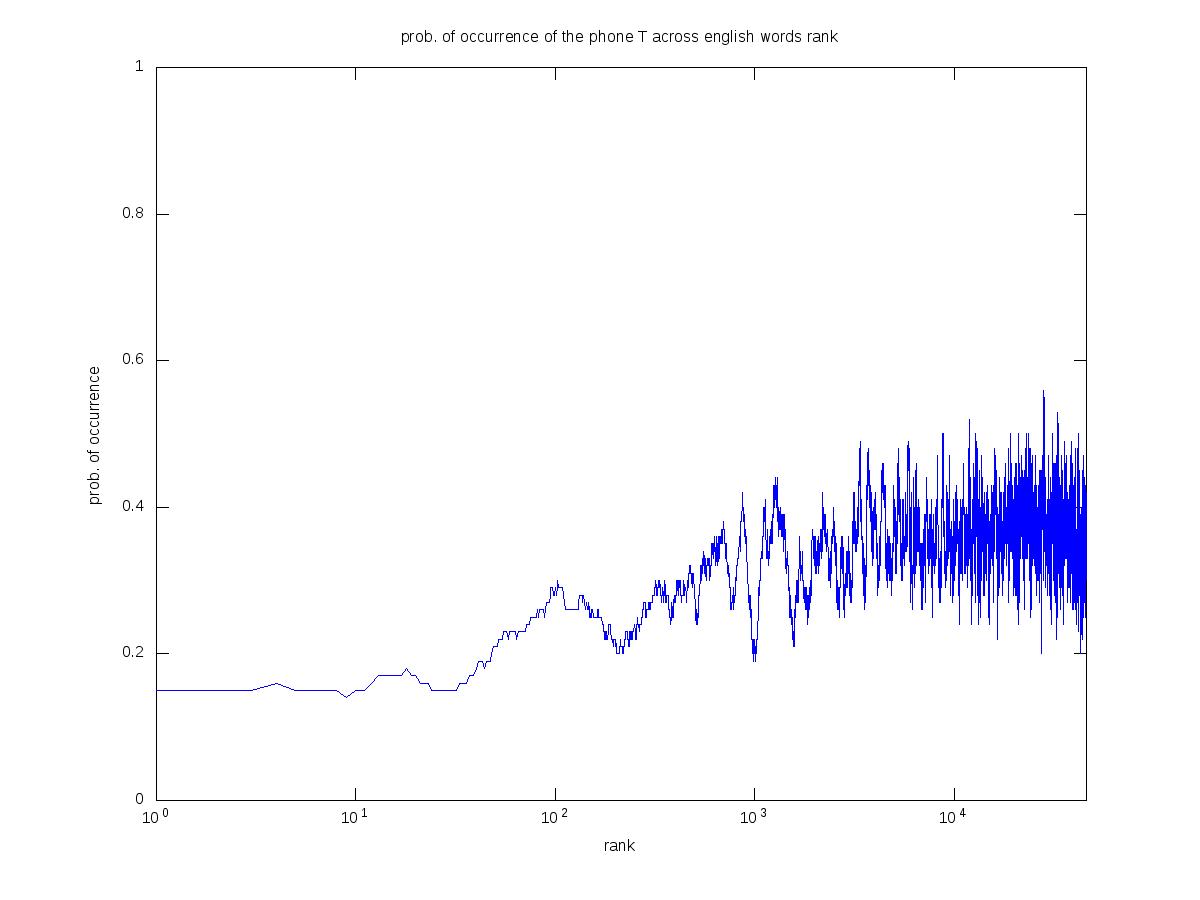
\includegraphics[width=0.45\textwidth]{images/proboccwordsphone_T.png}} \\
  \subfloat[Log-log plot of the frequency of occurrence of words with the phone \textipa{[f]} versus their rank.]{\label{fig:zipfwordsphone_F}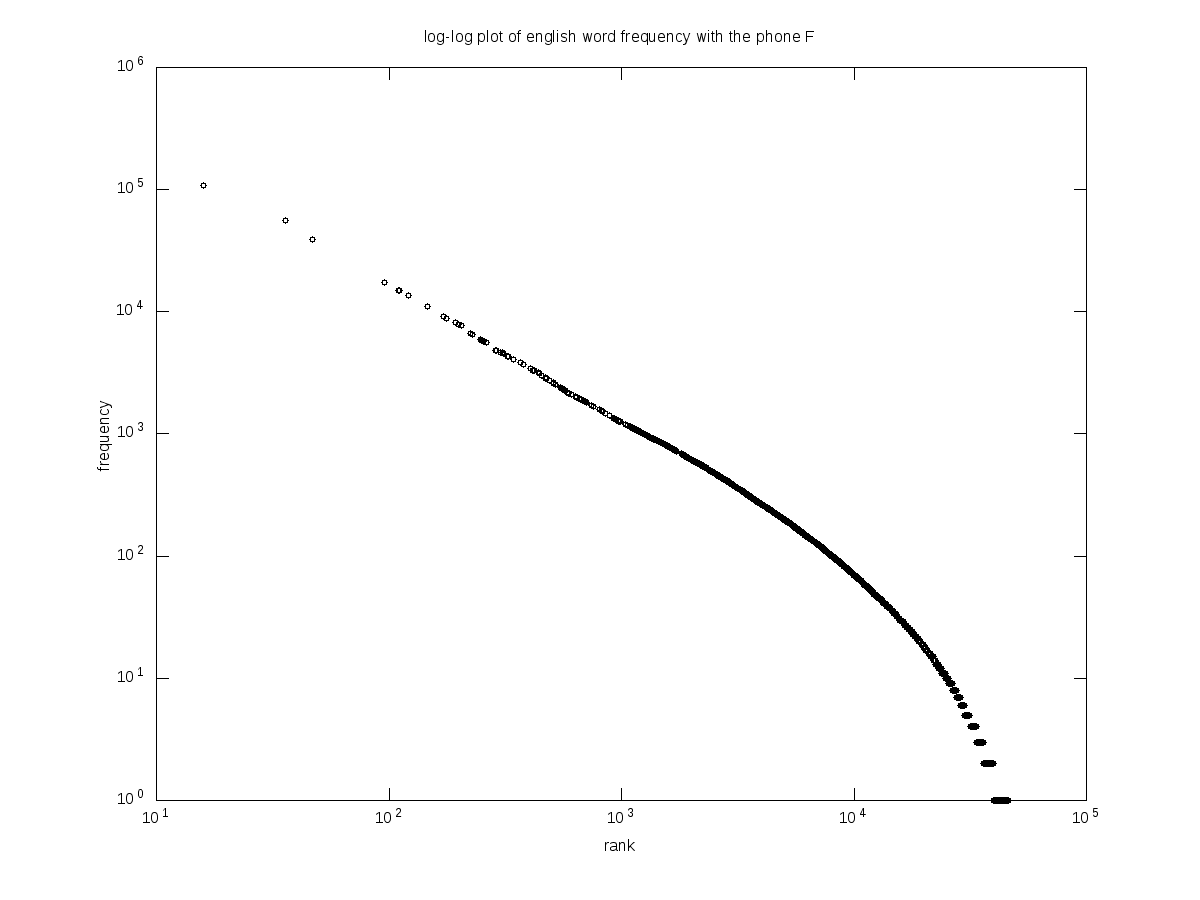
\includegraphics[width=0.45\textwidth]{images/zipfwordsphone_F.png}}
  \subfloat[Probability of occurrence of words with phone \textipa{[f]} versus the rank of words]{\label{fig:proboccwordsphone_F}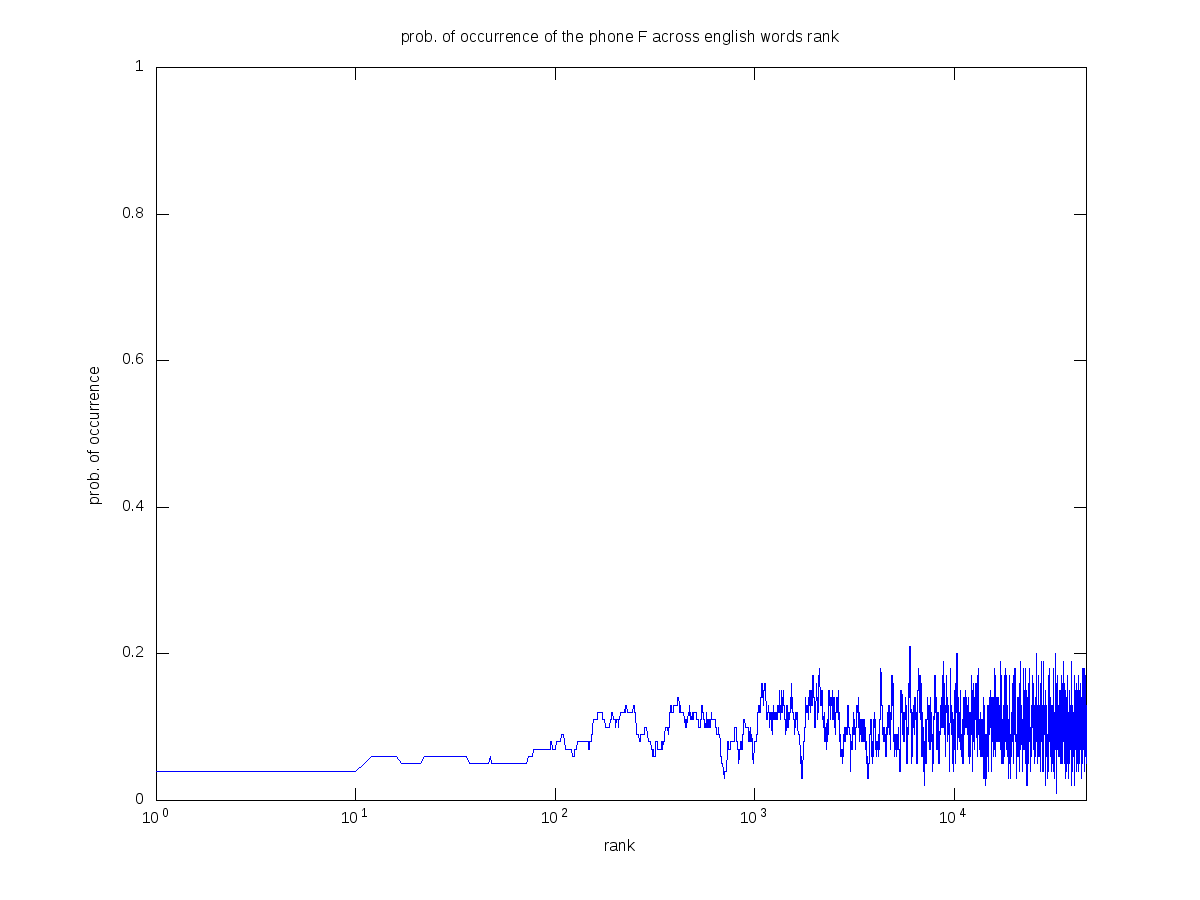
\includegraphics[width=0.45\textwidth]{images/proboccwordsphone_F.png}} \\
  \subfloat[Log-log plot of the frequency of occurrence of words with phone \textipa{[T]} versus their rank.]{\label{fig:zipfwordsphone_TH}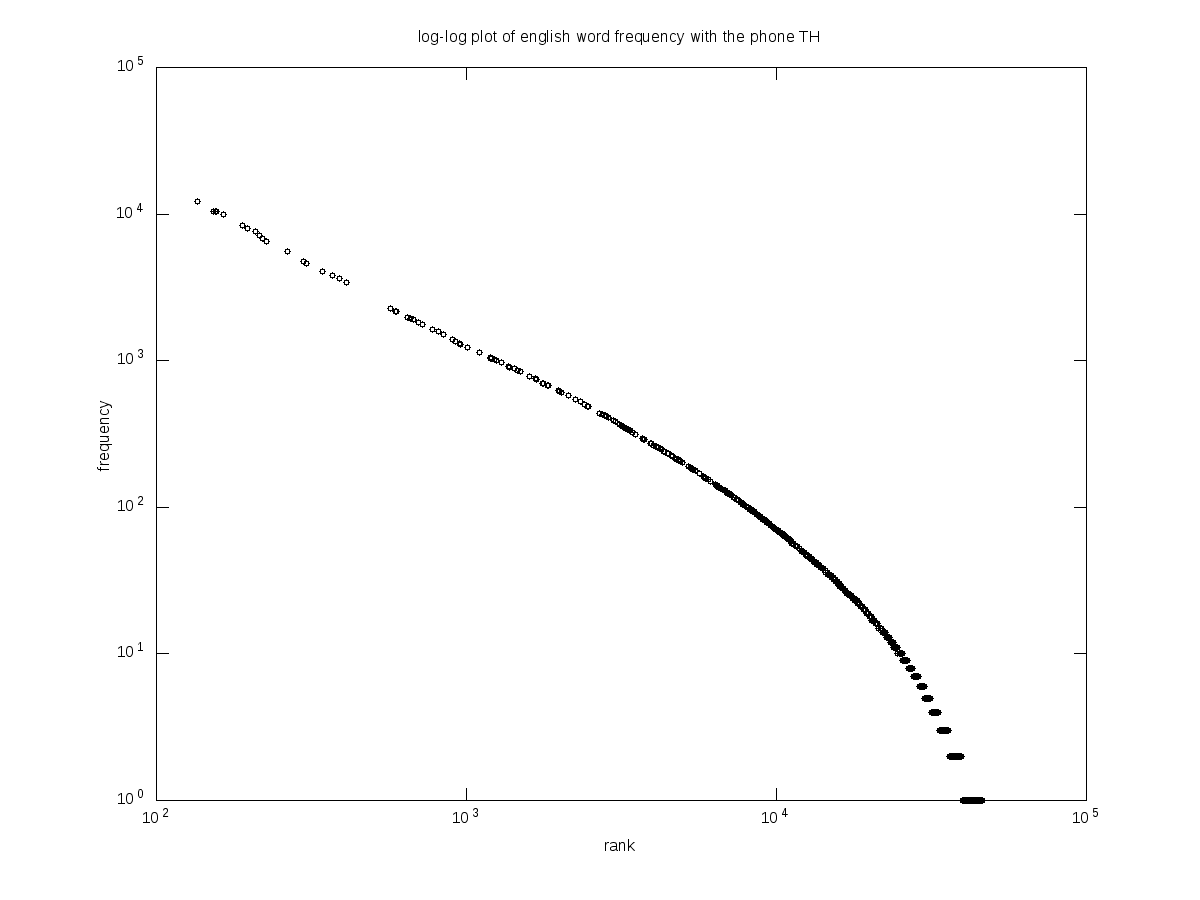
\includegraphics[width=0.45\textwidth]{images/zipfwordsphone_TH.png}} 
  \subfloat[Probability of occurrence of words with phone \textipa{[T]} versus the rank of words]{\label{fig:proboccwordsphone_TH}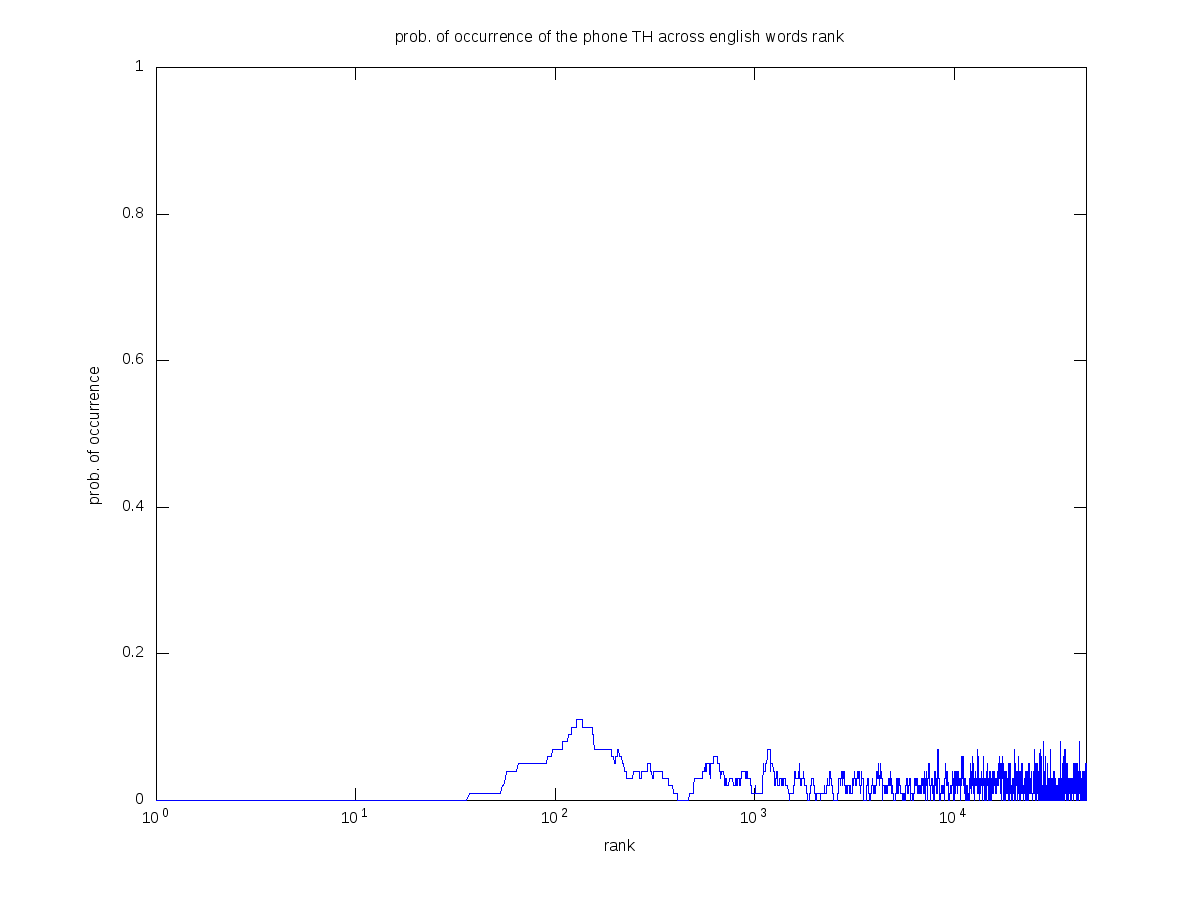
\includegraphics[width=0.45\textwidth]{images/proboccwordsphone_TH.png}} 
  \caption{Two types of graphics are presented to verify the contribution of word frequencies to the final phone frequencies. The left plot shows the occurrence of words with a certain phone. The right one shows an estimation of the probability of occurrence of a certain phone versus the rank of words.}
  \label{fig:wordszipfprobphone}
\end{figure*}



\begin{figure*}[p]
  \centering 
  \captionsetup[subfigure]{margin=10pt,singlelinecheck=false}
  \label{fig:wordsFreqIndexVsOccurrence}
  \subfloat[Each spot represents a word with a given frequency of occurrence and a frequency index. For a better visualization the frequency of occurrence is displayed in a logarithm scale.]{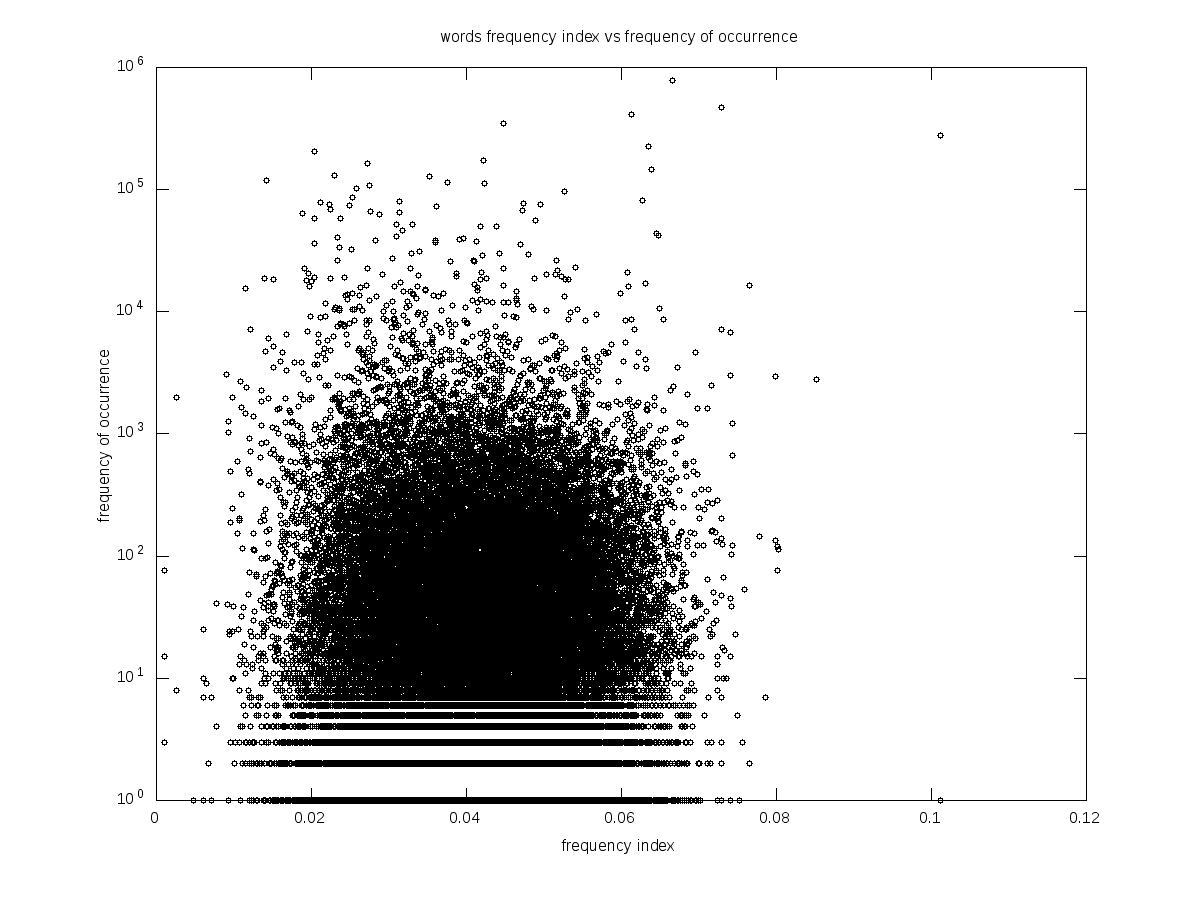
\includegraphics[width=0.45\textwidth]{images/wordsFreqIndexVsOccurrence.png}}                
  \subfloat[Density of words in each partition on the frequency of occurrence vs. frequency index space. The largest number is displayed in black and it refers to 578 words. White represents no word found in a spot. The gray scale is displayed in a logarithm fashion for better visualization.]{\label{fig:wordsFreqIndexVsOccurrenceDensity}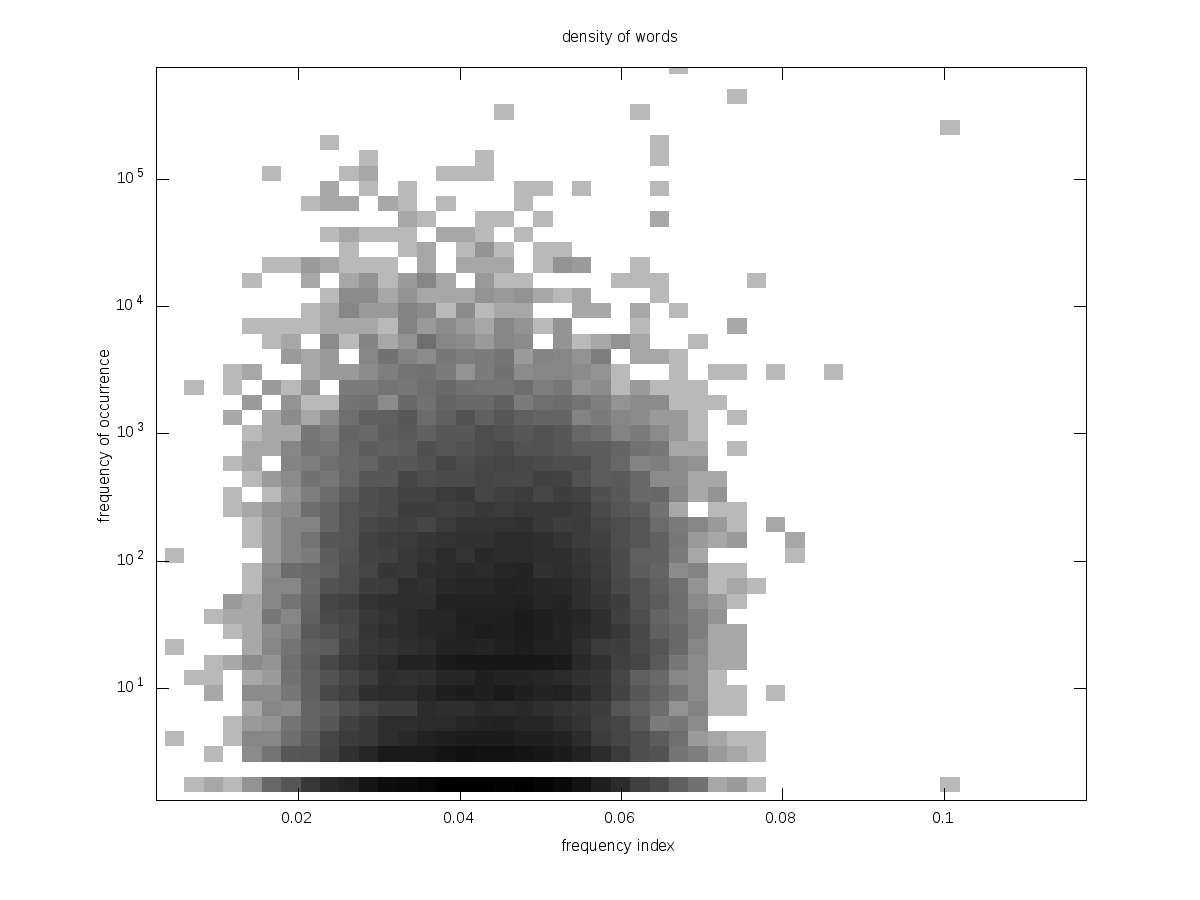
\includegraphics[width=0.45\textwidth]{images/wordsFreqIndexVsOccurrenceDensity.png}} 
  \caption{Relationship of word frequency of occurrence and word frequency index. The frequency index is the average probability of occurrence of the phones that make up the word.}
  \label{fig:wordsFreqIndexVsOccurrence12}
\end{figure*}


